\PassOptionsToPackage{table}{xcolor}
\PassOptionsToPackage{draft}{hyperref}
\documentclass[sigplan,10pt]{acmart}
\usepackage{enumitem}
\usepackage{booktabs} % For formal tables

\usepackage[utf8]{inputenc}
\usepackage{fullpage}

\usepackage{graphics}

\usepackage{graphicx}
\usepackage{subcaption}
\usepackage{nicefrac}
\usepackage{multirow}

%\usepackage{setspace}
\usepackage{ragged2e}
\usepackage{xspace}

	\usepackage{soul}

\usepackage{flushend}

%\usepackage{indentfirst}

\usepackage{amsthm}
\usepackage{amsmath,amssymb}
%\usepackage{mathrsfs}
\usepackage{mathtools}

\theoremstyle{definition}
\newtheorem{prop}{Proposition}[section]


%% Listing related stuff

\usepackage{listings}
\usepackage{courier}            %Required for pretty listings (more dense)
\usepackage{booktabs}

%% EMACS colors for listing:

\usepackage{color}
\definecolor{sh_comment}{rgb}{0.65, 0.00, 0.00 } % red-ish
\definecolor{sh_keyword}{rgb}{0.37, 0.69, 0.69}  % blue-green
\definecolor{sh_string}{rgb}{0.08, 0.69, 0.08} % green


\linespread{0.96}

%% This manipulates the listing numbering. It decreases it by one at the point used.
\newcommand*\lstDNumber{\addtocounter{lstnumber}{-1}}

%% Change from Listing->Algorithm
%% \renewcommand\lstlistingname{Algorithm} % Fix listing caption name: Listing -> Algorithm
%% \renewcommand\lstlistlistingname{Algorithms}
%% \def\lstlistingautorefname{Alg.}

%% \renewcommand{\thelstlisting}{\thesection-\arabic{lstlisting}}
%\renewcommand{\thelstlisting}{\arabic{lstlisting}} % Fix listing numbering Algorithm 1.1 -> Algorithm 1.

%% \renewcommand{\labelenumi}{\roman{enumi}.}

\lstset{
float=[*],
language=C,                % choose the language of the code
%% basicstyle=\linespread{0.9}
%% basicstyle=\scriptsize\ttfamily,
 basicstyle={\linespread{0.97} \scriptsize\ttfamily},
 stringstyle=\color{sh_string},
 keywordstyle = \color{sh_keyword}\bfseries,
 commentstyle=\color{sh_comment}\itshape,
numbers=left,                   % where to put the line-numbers
%% numberstyle=\scriptsize,        % the size of the fonts that are used for the line-numbers
numberstyle=\scriptsize,        % the size of the fonts that are used for the line-numbers
stepnumber=1,                   % the step between two line-numbers. If it is 1 each line will be numbered
numbersep=5pt,                  % how far the line-numbers are from the code
backgroundcolor=\color{white},  % choose the background color. You must add \usepackage{color}
showspaces=false,               % show spaces adding particular underscores
showstringspaces=false,         % underline spaces within strings
showtabs=false,                 % show tabs within strings adding particular underscores
xleftmargin=2em,                % Left margin
frame=lines,                   % adds a frame around the code. none|leftline|topline|bottomline|lines|single|shadowbox
framexleftmargin=1.5em,         % Margin from frame to line numbers
framexbottommargin=0em,         % Distance from last text to frame
morekeywords={in,true,false,and,or,set,is,not},
%% prebreak=\mbox{\tiny$\searrow$},
prebreak=\space,                % Line break: insert this character at the end of the top line
%% postbreak=\mbox{{\color{blue}\scriptsize$\hookrightarrow$}}, % Line break: blue arrow at the beginning of the bottom line
postbreak=\mbox{{\color{blue}\scriptsize$\hookrightarrow$}}, % Line break: blue arrow at the beginning of the bottom line
breaklines=true,                % sets automatic line breaking
breakatwhitespace=false,        % sets if automatic breaks should only happen at whitespace
tabsize=2,                      % sets default tabsize to 2 spaces
captionpos=b,                   % sets the caption-position to top
escapeinside={\@}{\@}             % Escape sequence \@ESCAPED STUFF\@
}

\usepackage{nasm/lang}
\usepackage{nasm/style}
\usepackage{llvm/lang}


% Copyright
\setcopyright{none}
%\setcopyright{acmcopyright}
%\setcopyright{acmlicensed}
%\setcopyright{rightsretained}
%\setcopyright{usgov}
%\setcopyright{usgovmixed}
%\setcopyright{cagov}
%\setcopyright{cagovmixed}


% DOI
%\acmDOI{10.475/123_4}

% ISBN
%\acmISBN{123-4567-24-567/08/06}

%Conference
\acmConference[CGO'18]{International Symposium on Code Generation and Optimization}{2018}{}
%\acmYear{1997}
%\copyrightyear{2016}
%
%\acmPrice{15.00}


\newcommand{\etal}{et~al.}

\newcommand{\itercomp}{{iterative compilation}\xspace}
\newcommand{\Itercomp}{{Iterative compilation}\xspace}
\newcommand{\IterComp}{{Iterative Compilation}\xspace}
\newcommand{\flagstype}{\usefont{T1}{cmr}{m}{n}}


\newcommand{\red}[1]{\textcolor{red}{#1}}
\newcommand{\blue}[1]{\textcolor{blue}{#1}}
\newcommand{\yellow}[1]{\textcolor{yellow}{#1}}
\newcommand{\green}[1]{\textcolor{green}{#1}}
\newcommand{\cyan}[1]{\textcolor{cyan}{#1}}
\newcommand{\brown}[1]{\textcolor{brown}{#1}}
\newcommand{\purple}[1]{\textcolor{purple}{#1}}
\newcommand{\orange}[1]{\textcolor{orange}{#1}}

\definecolor{Gray}{gray}{0.9}

\newcommand\FIXME[1]{\textcolor{red}{#1}}


\begin{document}
\title{Online {\IterComp}}

\author{ \vspace{2em} }

%\author{Rodrigo C. O. Rocha}
%\affiliation{%
%  \institution{University of Edinburgh, UK}
%}
%\email{r.rocha@ed.ac.uk}

%\author{Pavlos Petoumenos}
%\affiliation{%
%  \institution{University of Edinburgh, UK}
%}
%\email{ppetoume@inf.ed.ac.uk}

%\author{Lu\'is F. W. G\'oes}
%\affiliation{%
%  \institution{PUC Minas, Brazil}
%}
%\email{lfwgoes@pucminas.br}

%\author{Murray Cole}
%\affiliation{
%  \institution{University of Edinburgh, UK}
%}
%\email{mic@inf.ed.ac.uk}

%\author{Zheng Wang}
%\affiliation{%
%  \institution{Lancaster University, UK}
%}
%\email{z.wang@lancaster.ac.uk}

%\author{Hugh Leather}
%\affiliation{%
%  \institution{University of Edinburgh, UK}
%}
%\email{hleather@inf.ed.ac.uk}

%\renewcommand{\shortauthors}{R. Rocha et al.}

\begin{abstract}
    
    Iterative or adaptive compilation can dramatically improve the performance of a program by searching for the best optimization
    settings. However, it relies upon repeatedly evaluating and comparing optimizations off-line on predefined
    representative inputs. If the developers fail to guess what is a representative input or usage patterns change over time, 
    then the wrong optimizations may be selected. 
    Searching the optimization space with actual user inputs, during deployment, has previously seemed infeasible. 
    Program side effects, interactivity and difficulties capturing the system state mean that any given input can 
    only be executed once. Since each input may entail a different amount of work, the search cannot use runtime to compare 
    optimizations, and there is no baseline against which to define speedup.
    Unless we find a way to compare optimizations even when inputs are executed only once, we will be unable to use real user 
    input for iterative compilation, users will not have the best optimized programs, and performance and energy efficiency will suffer.
    
    We present metrics and techniques which, for the first time,  enable the use of true {\em online iterative compilation}.
    We compare optimizations by a new work efficiency metric, which requires only a single execution with any one input.
    We develop an instrumented, low overhead, mechanism for gathering the required data, using optimal probe placement in the source
    code. We show that overhead can be further reduced by removing high-cost probes whose absence introduces only small errors to the 
    work metric, without significantly affecting the outcome of the iterative compilation. 
    We give two variants for probe removal optimization: the first offers strong
    guarantees about the maximum possible error, while the second targets the average, whole program error.
    
    Our online iterative compilation method yields programs that get 80\% of the speedup achievable by an offline oracle, 
    but without executing any input more than once, which the oracle cannot do. 
    Through probe removal we bring the instrumentation overhead down to only 4\% on average, making our
    approach suitable for regular use. We show practical online iterative compilation for the first time, 
    optimizing programs according to the range of inputs users actually present.
    
\end{abstract}


%
% The code below should be generated by the tool at
% http://dl.acm.org/ccs.cfm
% Please copy and paste the code instead of the example below.
%
%\begin{CCSXML}
%<ccs2012>
%<concept>
%<concept_id>10011007.10011006.10011041</concept_id>
%<concept_desc>Software and its engineering~Compilers</concept_desc>
%<concept_significance>500</concept_significance>
%</concept>
%<concept>
%<concept_id>10011007.10011006.10011041.10011043</concept_id>
%<concept_desc>Software and its engineering~Retargetable compilers</concept_desc>
%<concept_significance>500</concept_significance>
%</concept>
%</ccs2012>
%\end{CCSXML}

%\ccsdesc[500]{Software and its engineering~Compilers}
%\ccsdesc[500]{Software and its engineering~Retargetable compilers}
\keywords{{\IterComp}, Profiling} %, Relaxed Instrumentation}

\maketitle
\vspace{-1em}

\vspace{-2em}
\section{Introduction}

Modern optimising compilers have reached a high level of sophistication,
providing a large number of optimisations, where the correct choice of
optimisations and their ordering can have a significant impact on the
performance of the code being optimised.
Although compilers offer a set of prearranged optimisation sequences that are
expected to yield reasonable improvements in many programs, there is still the
potential for performance degradation for certain programs, as these
optimisation sequences do not include all possible optimisations and are always
applied in the same pre-defined order, without regard the code being
optimised~\cite{pan06,cavazos07,zhou12,kulkarni12}.
A well-known compilation technique that addresses this challenge is {\itercomp},
which has the ability to adapt to new platforms, program and workload while
still having a systematic and simple optimisation process~\cite{kisuki99,fursin07,chen10}.
%It works by repeatedly evaluating a large number of optimisation sequences until
%the best combination is found for a particular
%program~\cite{kisuki99,fursin07,chen10}.

%{\Itercomp} is a well-known compilation technique that addresses the problem of
%efficiently selecting the best optimisation sequence for a given program.
%Although compilers offer a set of prearranged optimisation sequences that are
%expected to yield reasonable improvements in many programs, there is still the
%potential for performance degradation for certain programs, as these
%optimisation sequences do not include all possible optimisations and are always
%applied in the same pre-defined order, without regard the code being
%optimised~\cite{pan06,cavazos07,zhou12,kulkarni12}.
%{\Itercomp} have a systematic and simple optimisation process, where it works
%by repeatedly evaluating a large number of optimisation sequences until the best
%combination is found for a particular program~\cite{kisuki99,fursin07,chen10}.

However, until recently, most of the existing work in {\itercomp} had been focusing on
finding the best optimisation through repeated runs using a single input.
Although they demonstrate the potential of {\itercomp}, in real-world
\textit{online} scenarios the user rarely executes a program with the same input
multiple times~\cite{bodin98,kisuki99,stephenson03,kulkarni04,agakov06}.
Furthermore, most of real-world programs are complex enough so that a single
input case does not capture the whole range of possible scenarios and program
behaviours~\cite{haneda06,fursin07,chen10,chen12a}.
Because programs can exhibit behaviours that differ greatly depending on the
input, using a single input for {\itercomp} may not result in a good performance
when executing the optimised code with different inputs.

The main goal of this paper is to enable {\itercomp} in online scenarios.
We define the online scenario as having the restriction that programs execute
multiple inputs and distinct inputs are executed only once.
This online aspect is usually found in mobile and data centre
platforms~\citep{chen12b,fang15,mpeis16}, where the goal is to optimise programs
to consume less resources based on the workload of a particular user or group of
users.

Because of the restriction of having a single execution per input, it is not
possible to measure speedup for comparing optimisations.
Moreover, measuring just execution time, for example, is also not viable since
different inputs often mean different amounts of work,
rendering it meaningless to compare optimisations only by execution time.
%amount of work is often expected to differ between 
%useful only if the
%amount of work is constant between executions with different inputs.
Similarly, although previous works have suggested using
\textit{instructions per cycle} (IPC) for performing {\itercomp} in online
scenarios, IPC also have no correlation with speedup~\citep{fursin07}.

In order to tackle this problem, we propose the a work-efficiency metric that
enables to compare the performance of different optimisations using executions
of the program with distinct inputs.
It works by instrumenting the program, in optimally selected places, using a
single global counter which measures the amount of work the program performed
during its execution.
Equiped with this work metric, we are able to compute the work-efficiency
performance using a single execution of an optimised version of the program,
which can then be used to guide online {\itercomp}.

We acknowledge that having a low-overhead profiling for the work-efficiency
metric is essential in this online scenario for two main reasons:
$(i)$ the user is directly affected by large overheads;
$(ii)$ a highly intrusive instrumentation can have significant impacts on the
effect of optimisations, due to complex and unpredictable decisions taken by
many of the compiler's heuristics.
With the purpose of reducing the profiling's overhead, we propose two relaxation
algorithms which provide a trade-off between measurement accuracy and overhead.
%The first is a relaxation algorithm that operates on the level of regions of
%functions, while the second performs the relaxation considering the whole
%program at the same time.
These relaxation algorithms are able to reduce the overhead by incurring very
small and bounded percenage errors in the measurement of work.
The benefits of reducing the overhead often outweighs the inaccuracy introduced,
because of the two aforementioned drawbacks of large overheads.

Our evaluation shows that performing online {\itercomp} guided by work efficiency
achieves about 80\% of the performance of an offline oracle, with improvements
of up to about 20\% over the compiler's standard optimisation.
While our solution executes each input a single time to measure the work
efficiency metric, the offline oracle is allowed to execute multiple times to
have a statistically sound measurement of the actual speedup.
Regarding the two relaxation algorithms, our results show an average reduction
in overhead of 43\% and $2.1\times$ over the optimal work profiling, observing
up to about $5\times$ of overhead reduction, while often incurring in much less
than 1\% of dynamic error in the measurement of work.

%Our experimental evaluation shows that performing online {\itercomp} guided by the work-based performance (WP) metric good results compared to the oracle, which is allowed to execute each input multiple times in order to use the actual speedup for guiding the {\itercomp}.
%Online {\itercomp} guided by the WP metric is able to achieve an average of 7.5\% and a maximum of 33\% improvement over the standard {\flagstype -O3} optimisation.
%Moreover, the experiments regarding the work profiling show that both relaxation algorithms are able to significantly reduce the profiling overhead while incurring a dynamic error of less than 5\% in the work measurement.
%The whole program relaxation achieves an average of $2\times$ reduction in the overhead compared with the optimal profiling technique, while the more conservative relaxation that operates per region achieves an average improvement of 40\% over the optimal profiling.

%Our main contributions are the following:
%\begin{itemize}
%\item The use of a work-based performance metric in order to enable \textit{online} {\itercomp} by comparing different combination of compiler optimisations even when executed with distinct inputs.
%\item We propose a relaxed instrumentation for low overhead profiling, with a controlled trade-off between accuracy and overhead.
%\end{itemize}

To summarise, the main contributions of this paper are the following:
\begin{itemize}
\item We propose a work efficiency profiling that measures a performance rank
of an optimised program using a single execution.
\item We show the effectiveness of the work efficiency for guiding {\itercomp} in an
online scenario, where the program is expected to execute only once for distinct
inputs.
%\item Contrary to what previous work has suggested, we show that instructions per cycle (IPC) is not a good metric for online {\itercomp}.
%\item We adapt the block frequency profiling in order to measure the WP metric.
\item A conservative relaxation algorithm is proposed for reducing the overhead of the work profiling, with a guaranteed bound for the error.
\item A more aggressive relaxation algorithm is proposed, which works on the whole program, in order to further reduce the overhead of the work profiling.
\end{itemize}

\section{Motivation \label{sec:motivation}}

    In this section we first motivate online iterative compilation by showing the deleterious effects of choosing the wrong inputs for the
    offline case. Then we go on to show the unsuitability of previously proposed program version comparison metrics.

    \begin{figure}[t!]
        \centering
        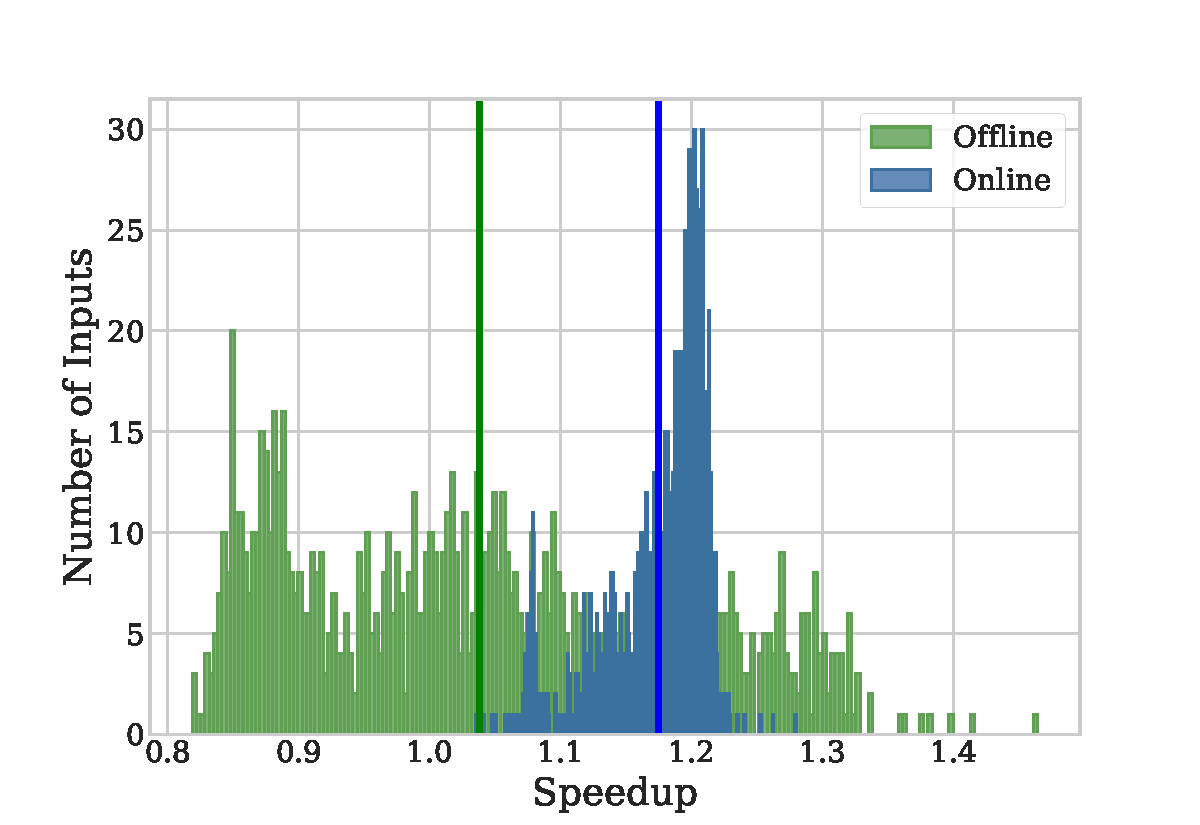
\includegraphics[width=0.5\textwidth]{figs/motivation-online.pdf}
        \caption{
            Histograms of speedup over \texttt{-O3} for each of the 1,000 inputs of \texttt{susan\_c}. The green histogram shows the
            speedup when using the optimization sequence selected by offline \itercomp, the blue one is the speedup using the optimization
            sequence selected by an online-like approach.
        }
        \label{fig:motivation-online}
    \end{figure}

    We performed offline iterative compilation on the \texttt{susan\_c} benchmark to find the optimization settings that maximize the average performance
    over five randomly chosen inputs from a set of 1,000 provided by the \textit{KDataSets} benchmark suite~\cite{chen10,chen12a}.
    The green histogram in Figure~\ref{fig:motivation-online} shows, for each of the 1,000 inputs, the speedup versus \texttt{-O3} of that
    chosen optimization setting. The dark green line shows the average speedup for all those inputs. The five training inputs are
    all among the top performing inputs. On the other hand, the chosen optimization does poorly on other inputs, often causing
    a slowdown and yielding only a slight speedup of 4\% on average.

    The blue bars in Figure~\ref{fig:motivation-online} show a different approach. Here the iterative compilation proceeds by evaluating
    each optimization on five inputs. Each input is evaluated only once during the search, but the search is provided with oracle
    knowledge about the unoptimized runtime for the inputs, giving a perfect speedup metric. The environment of the search constantly
    changes in the same way as for online iterative compilation. The best optimization for this case never degrades performance compared to
    \texttt{-O3} and is on average 13\% better than the offline approach. The online case, considering truly representative inputs, leads
    to superior performance, if the speedup caused by optimizing can be estimated.

    \begin{figure}[t]
        \centering
        %\begin{tabular}{cc}
        %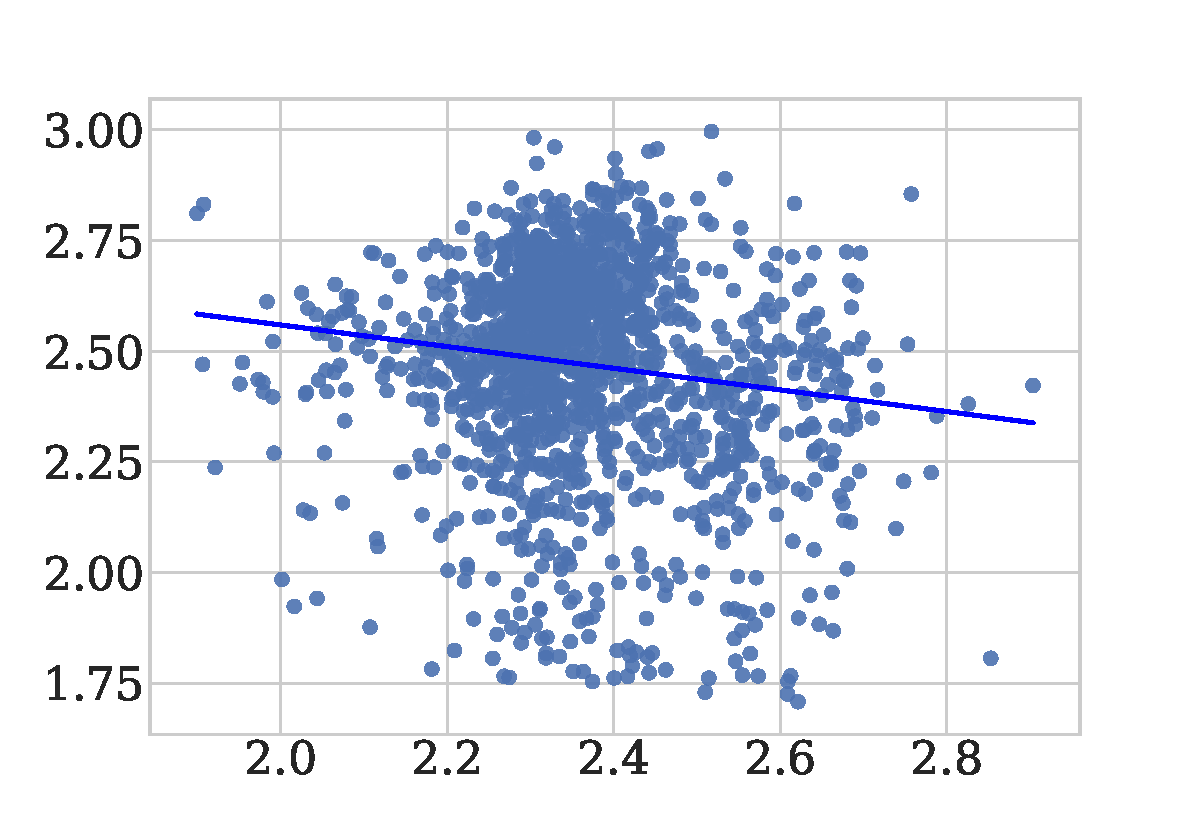
\includegraphics[width=0.25\textwidth]{figs/motivation-metric-ipc.pdf} &
        %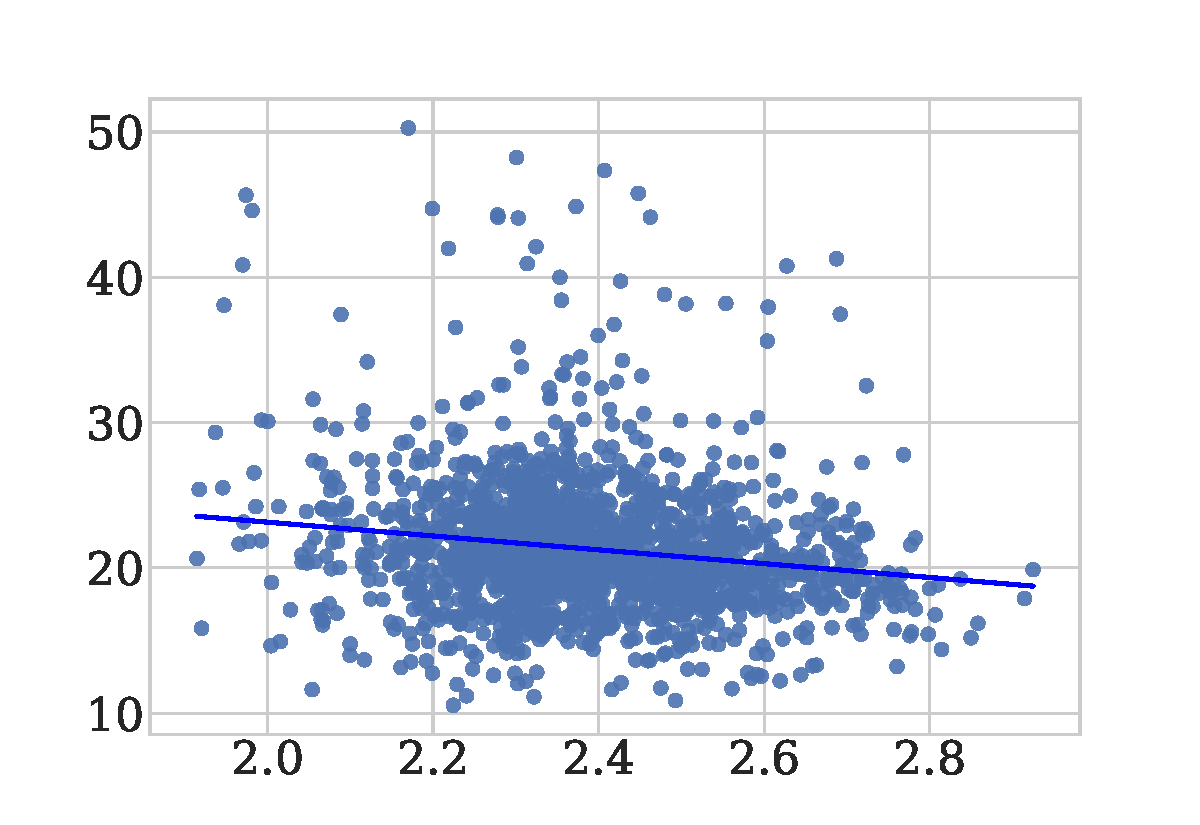
\includegraphics[width=0.25\textwidth]{figs/motivation-metric-runtime.pdf}
        %\end{tabular}
        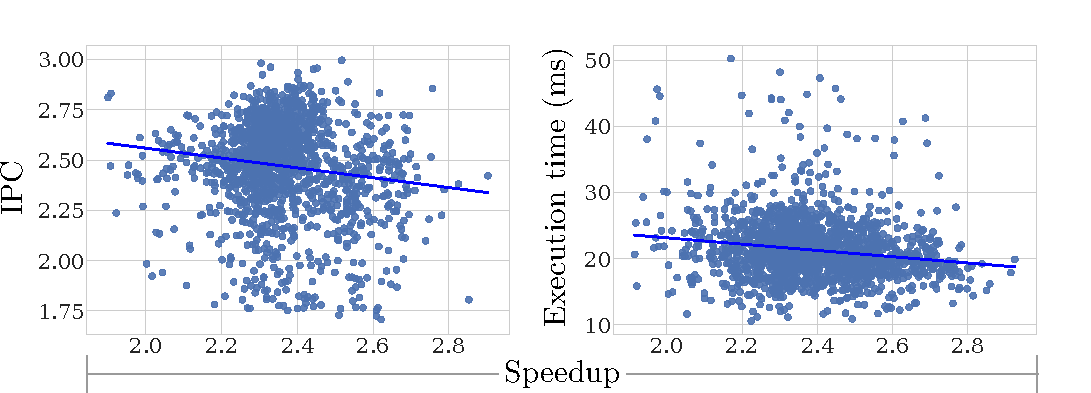
\includegraphics[width=0.5\textwidth]{figs/motivation-metric.pdf}
        \caption{
            Relationship between IPC and execution time \textit{vs} speedup over the unoptimized program
            for 500 different binaries of \texttt{susan\_c}.
            Each point represents the average over a subset of all inputs.
            The IPC and execution time show correlation coefficients of $-0.14$ and $-0.16$, respectively.
        }
        \label{fig:motivation-metric}
    \end{figure}

    Prior to this paper there were two proposed metrics to correlate with program efficiency. The first is simply to use runtime, ignoring
    the work aspect. This functions well when the inputs all require similar effort. When that is not the case it bears little or no
    correlation to efficiency. The second approach is \textit{instructions per cycle}~(IPC), suggested by~\citep{fursin07}. While IPC seems
    promising in the sense that faster instruction execution is a good thing, this is belied by the simple observation that adding
    redundant NOPs to a program will increase IPC while also slowing the program down. Figure~\ref{fig:motivation-metric} shows the
    relationship between execution time, IPC and speedup for different optimizations of \texttt{susan\_c}, averaged across a subset of the
    inputs. We use correlation coefficient~\cite{Bishop:2006:PRM:1162264} to quantify if  IPC and execution time are strongly correlated to
    speedup.
    %This correlation coefficient takes a value between -1 and 1, the closer the coefficient is to +/-1, the stronger the
    %correlation between the variables.
    In our case, the IPC and execution time show correlation coefficients of $-0.14$ and $-0.16$,
    respectively, to speedup.
    %These values are far from 1, suggesting that there is a weak correlation between speedup and IPC or execution time.
    Neither IPC nor execution time correlate well, and so neither can be used for iterative compilation. We need a work efficiency
    metric which can approximate speedup instead, using only a single execution.

    In the remainder of this paper we present our work efficiency metric and demonstrate its utility for iterative compilation.

\section{Work Efficiency} \label{sec:work}

    In this section, we introduce \textit{work efficiency}, a novel performance metric for comparing the quality of different optimized
    versions of a program, even when we evaluate them with a different input each time. Similarly to existing one-shot performance metrics,
    work efficiency is simply the amount of \textit{work done per unit of time}: 
    \[
        \textrm{Work Efficiency} = \frac{\Delta W}{\Delta t}
    \]
    where $\Delta W$ is the amount of work performed during a period of time $\Delta t$.

    With similar metrics, what exactly is work depends on the application and is defined by the developer: SQL queries executed,
    transactions completed, bytes processed, etc. In our case, we need a similar but application-agnostic metric which correlates with what
    the developer considers useful work and is simple enough to be calculated online.

    Section~\ref{subsec:workmetric} describes this new work metric and the design choices we made, Section~\ref{subsec:prof} details how
    we measure work, and Section~\ref{subsec:relaxed} explores ways to measure it with reduced interference on %without interfering with
    the normal operation of the program.

    \subsection{Work Metric} \label{subsec:workmetric}

    To build a reasonable work metric, our approach starts by assuming that each executed instruction\footnote{In this paper, we consider instructions at the level of the Intermediate Representation (IR) of the LLVM compiler.} contributes a certain amount towards
    the total useful work. To keep the measurement simple and minimize the online overhead, we assume that the contribution depends only on
    the type of instruction. Additionally, we would expect two program versions processing the same data in the same way to do the same
    work. If measured using the actual instructions executed for the two versions, we would get a different amount of work. Instead, we
    increase the total work based on the instructions that would be executed with the unoptimized code, regardless of the version we use.
    The unoptimized version is convenient as a common baseline, since we start with it anyway and it is as close as possible to the
    programmer's intention.

    We selected the work contribution of each instruction type so that total work becomes an estimator of the runtime of the unoptimized
    program.
    %Our choice to associate work with unoptimized runtime is largely arbitrary but instinctively reasonable.
    Our choice to associate work with unoptimized runtime is largely for practical reasons but it is also instinctively reasonable.
    Unoptimized time is
    close to how the programmer understands the effort put by the computer. Using it as the work metric makes work efficiency (work per unit
    of time) an estimator of the speedup of the optimized version over the unoptimized version. While other ways of setting the instruction
    contributions might be better, our results in Section~\ref{sec:results} show that this simple definition of work produces good results.
    Using the experimental setup described in Section~\ref{sec:setup}, we run the unoptimized versions of the 10 benchmarks listed in
    Table~\ref{tab:kdatasets:training} with all 1,000 available inputs. For each run, we recorded execution time and dynamic counters for all instruction types\footnote{
    Dynamic instruction counts were obtained by using the classic block-frequency profiling.}.
    Similarly to prior work~\cite{giusto01,powell09,brandolese11}, we then applied linear regression to find the contribution of each
    instruction type that minimizes the error between measured runtime and work.
    %\footnote{The resulting regression model uses \FIXME{70}
    %different instruction types which make it too long to present here.}

%%    \begin{figure}[t]
%%        \centering
%%        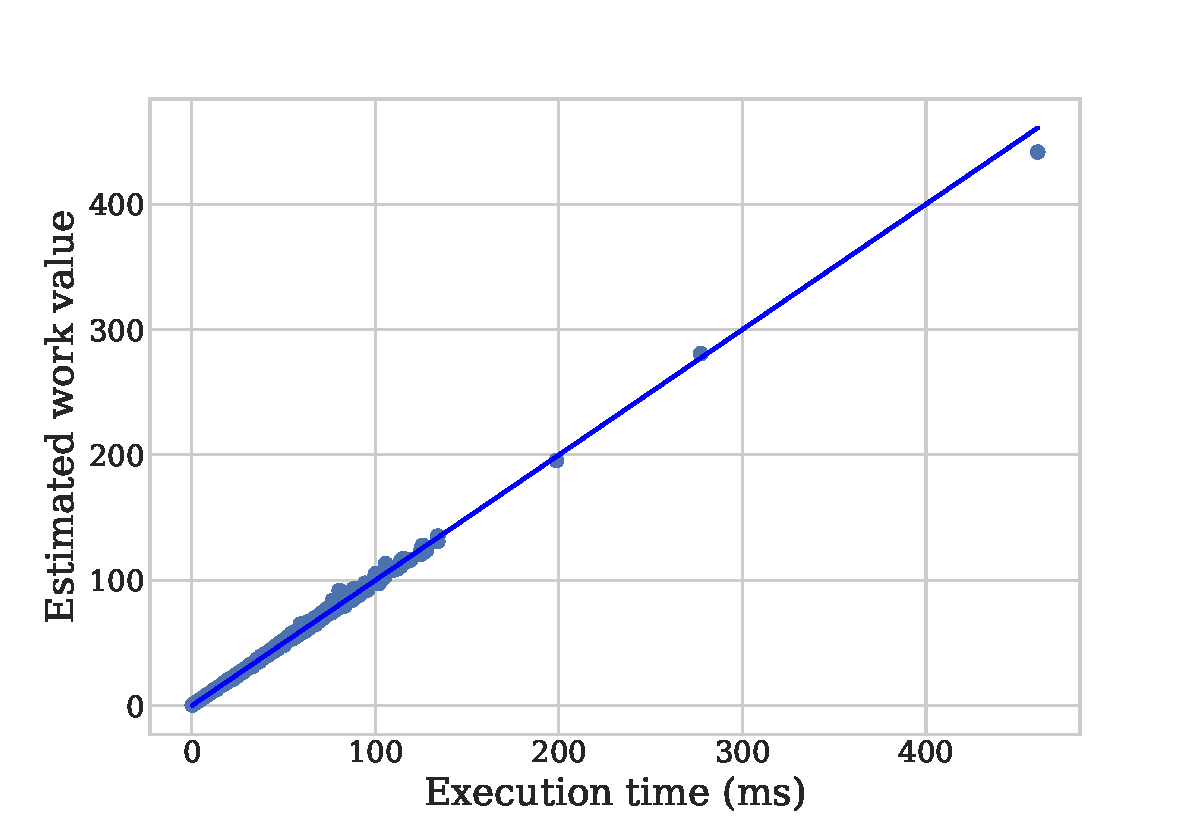
\includegraphics[width=0.5\textwidth]{figs/work-correlation-with-O0_susan_c.pdf}
%%        \caption{
%%            Relationship between work metric ($\Delta W$) and the execution time of the unoptimized version of the \texttt{susan\_c}
%%            benchmark over the 1,000 inputs. Each point represents the execution of a single input. They have a correlation coefficient of
%%            $0.99$.
%%        }
%%        \label{fig:work-vs-O0time}
%%    \end{figure}
    
    Figure~\ref{fig:work-vs-O0time} shows the correlation coefficient between the work metric ($\Delta W$) and the runtime of the
    unoptimized version for 14 benchmarks that were not used for training the linear model. The work metric correlates very strongly with
    runtime for almost all the benchmarks, the correlation coefficient being typically higher than $0.98$. The exception is the benchmarks
    based on \texttt{tiff}. The coefficient for them ranges from $0.47$ to $0.96$. Despite that, in most cases work is an excellent proxy
    for unoptimized runtime. For the rest, our Section~\ref{sec:results} evaluation shows that our work metric is still useful for quantifying
    performance. 


\begin{figure*}[t]
    \centering
    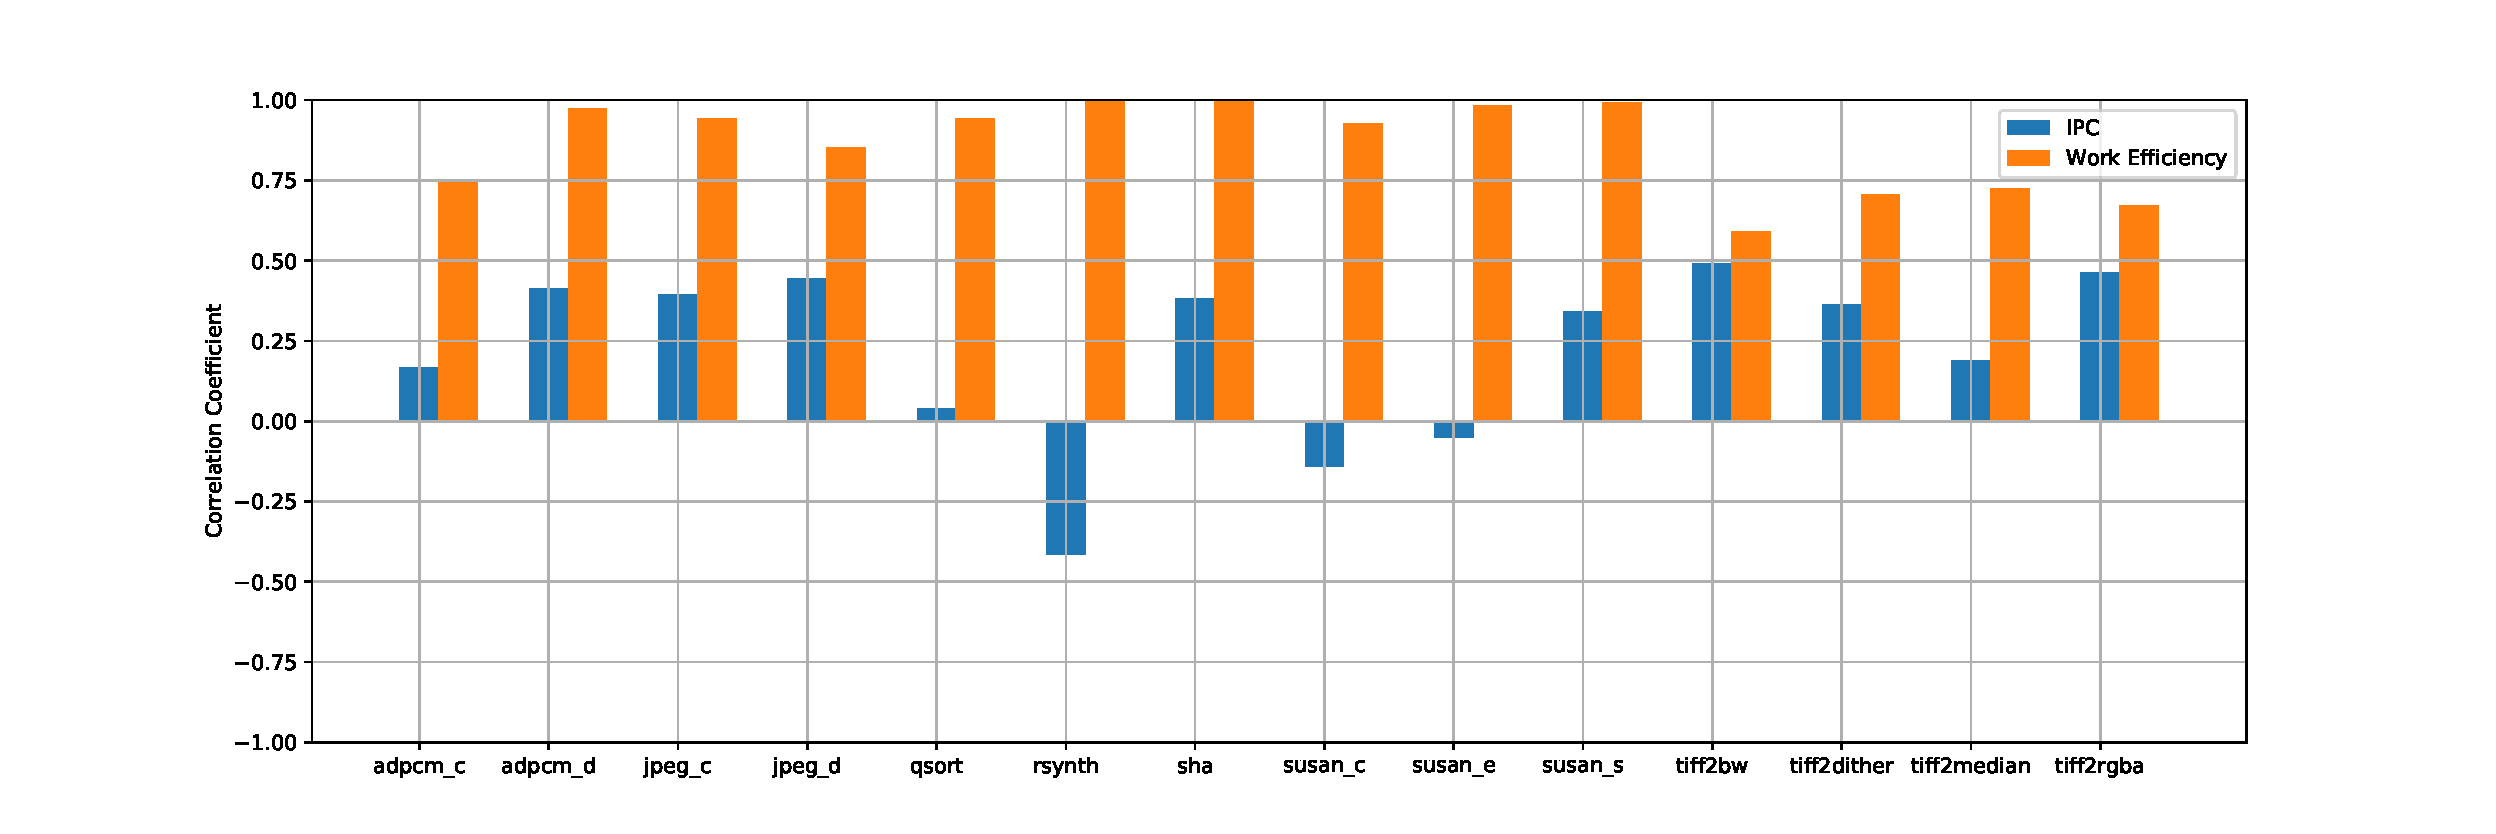
\includegraphics[width=\textwidth]{figs/corr_coeff.pdf}
    \caption{Correlation coefficients between the work metric ($\Delta W$) and the execution time of the unoptimized version for each benchmark.}
    \label{fig:motivation-speedups}
\end{figure*}


    \subsection{Work Profiling}\label{subsec:prof}

    Total work is just the sum of the cost of all instructions that would be executed in the unoptimized binary. A na\"{\i}ve but
    straightforward way to measure work online is to instrument the unoptimized code with a global work counter and instructions for
    incrementing this counter after each instruction of the original code. Since the work contribution of each instruction depends only on
    its type, it can be determined at compile time. Taking this one step further, we can calculate work contributions at the basic block
    level and insert only a single increment instruction in each block. Although easy to implement, the na\"{\i}ve approach introduces a
    significant overhead.

    Previous work on basic block profiling has proposed ways for instrumenting the code with as little overhead as possible without losing
    any profiling information~\cite{knuth73,ball94}. The underlying idea is that we can still calculate precisely the execution counts of
    all basic blocks if we choose a spanning tree of the function Control Flow Graph (CFG) and only instrument the edges of the CFG
    \textit{not} in the tree~\cite{nahapetian73,forman81}. To make the instrumentation probe placement optimal, we choose the maximum
    spanning tree, with the edge weights representing edge frequency estimates. This maximises the number of high frequency edges that will
    not be instrumented, minimizing the instrumentation cost~\cite{forman81,ball94}. 
    
    \begin{figure}[t]
    \centering {
      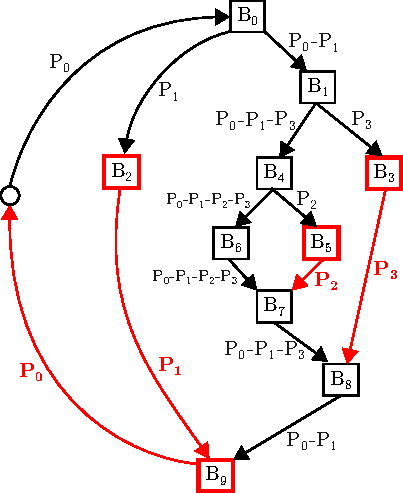
\includegraphics[scale=0.8]{figs/cfg-example.pdf}\\\vspace{1ex}
      \resizebox{0.45\textwidth}{!}{
      %\scalebox{0.8}{
         \begin{minipage}{0.5\textwidth}
         Instrumented value for each probe $P_i$:
         \begin{align*}
         \omega(P_0) &= w(B_0) + w(B_1) + w(B_4) + w(B_6) + w(B_7) + w(B_8) + w(B_9)\\
         \omega(P_1) &= w(B_2) - w(B_1) - w(B_4) - w(B_6) - w(B_7) - w(B_8)\\
         \omega(P_2) &= w(B_5) - w(B_6)\\
         \omega(P_3) &= w(B_3) - w(B_4) - w(B_6) - w(B_7)
         \end{align*}
         \end{minipage}
      }
    }
      \caption{Example of a CFG with its maximum spanning tree in black. Basic blocks and edges highlighted in red are instrumented.
        Instrumenting them is enough for calculating the total work performed by the whole CFG.}
      \label{fig:cfg-example}
    \end{figure}

    With na\"ive instrumentation each basic block records only its own amount of work. With optimal probe placement, reaching a probe
    implies not only executing the containing block but also executing or not executing other uninstrumented blocks, so work counter
    increments have to reflect this. Figure~\ref{fig:cfg-example} shows an example CFG, where the instrumented blocks are marked with red.
    In this example, reaching probe $P_2$ implies not only executing block $B_5$ but also not executing $B_6$.
    
    To compute the amount of work associated with each instrumentation probe, we first need to determine how reaching a probe relates with
    executing or not a basic block. Starting from instrumented edges, we use Kirchhoff's first law~\cite{knuth73,ball94} and a post-order
    traversal of the spanning tree to build symbolic expressions of edge frequencies as linear functions of probe counts, as seen in
    Figure~\ref{fig:cfg-example}. This part is identical to how edge and block frequencies are calculated in prior work for basic block
    profiling.
    
    %Simply put, the sum of the frequencies of the edges entering a block and the sum of the frequencies
    %exiting the same block must match. Starting from the leaf nodes of the spanning tree, where by definition all edges except one should
    %be instrumented, and working upwards, we should be able to calculate the frequencies of all nodes and edges as a function of the probe
    %of the probe counts.
    
    If a block's frequency expression contains a positive term for a probe, this means that the block is executed when we reach the probe,
    so the block's cost should be added at that probe. Conversely, if the expression contains a negative term for a probe, then the block
    is executed when we do not reach the probe, so the block's cost should be subtracted. In our example CFG, the symbolic expression for
    the basic block $B_8$ is $P_0 - P_1$, so the amount of work of $B_8$, denoted by $w(B_8)$, is incremented in probe $P_0$ and
    decremented in $P_1$.


    \subsection{Relaxed Instrumentation}\label{subsec:relaxed}

    Optimal instrumentation significantly reduces the profiling overhead when compared to na\"ive instrumentation, from an average overhead
    of 79\% to 13\%. Still, 13\% slowdown might be more than what the user is ready to tolerate, while for isolated case the overhead might
    be as high as 60\%. We need to reduce overhead further to make the work metric practical. 
    
    We propose two novel relaxation strategies that offer a trade-off between accuracy and overhead. Our insight was that, unlike basic
    block profiling, not all probes are of equal importance. The work associated with some is insignificant compared to the total work
    done by the program, so ignoring them will have little negative impact on the accuracy of measuring work. By removing such probes,
    especially if they are frequently executed, we can reduce the instrumentation overhead dramatically. These two strategies are
    particular to work profiling and reduce the overhead much more than what previous research in basic block profiling has achieved. 

    To select which probes to remove we consider the probes in a control flow region. The runtime benefit of removing a probe is
    proportional to the frequency of the block the probe is in, while the error introduced is proportional to both the work contribution of
    the probe and its frequency. We solve the 0-1 Knapsack optimization problem, removing probes to maximize the total savings while
    keeping the accumulated error below a threshold:
    \begin{gather*}
        \textrm{max.}\quad\sum_{i=0}^{k} f(P_i)x_i,\quad
        \textrm{s.t.}\quad\sum_{i=0}^{k} \varepsilon(P_i)x_i \leq M \\
        x_i\in\{0,1\}, i\in\{0,\ldots,k\}
    \end{gather*}
    where the set of probes in the region being considered is $\{P_0, P_1, \ldots, P_k\}$, $f(P_i)$ is the execution frequency of probe
    $P_i$ and $x_i$ denotes the probes selected for removal, $\varepsilon(P_i)$ is the error for removing $P_i$ and $M$ is the maximum
    error threshold.

    For our experiments, we implemented two solvers for the 0-1 Knapsack problems: an optimal but potentially slow brute-force solver and a
    greedy heuristic based on sorting the items~\cite{dantzig57}. We use the brute-force solver with a small number of probes, less than
    20, and the greedy heuristic otherwise.

    We have two relaxation strategies which differ in the control flow regions they tackle and how they calculate the error terms. The
    first is a more conservative approach that calculates induced error from removing a probe by considering the worst case of any
    execution path through the program. The second is a more aggressive approach that computes induced error based on the relative change
    of the work measurement that removing a probe would make to the total amount work for the whole program. We discuss each one of them
    in detail.

    \subsubsection{\WCRelaxTitle Relaxation}

    In order to offer hard guarantees for the error upper bound, this conservative approach first decomposes the CFGs of the program into
    subgraphs where the maximum possible work contributed by each probe, as well as the minimum possible amount of total work for the whole
    subgraph, can be calculated. Then, it removes probes within each subgraph while keeping the maximum possible error rate for that
    subgraph bounded by the threshold. With the error rate of each subgraph below the threshold, it is guaranteed that the dynamic error of
    the work metric for the whole program will always be bounded by the threshold.

    \begin{figure}[t]
      \centering
      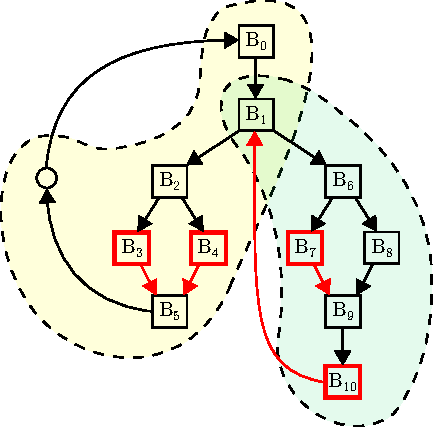
\includegraphics[scale=0.8]{figs/cfg-relax-example.pdf}
      \caption{Example of a CFG containing a loop and its decomposition into DAGs.
               The DAGs are the subgraphs within the dashed boundaries.}
      \vspace{-4mm}
      \label{fig:cfg-relax-example}
    \end{figure}

    The \WCRelaxLower relaxation starts by extracting directed acyclical graphs (DAGs) from the CFG. The algorithm extracts subgraphs that
    represent loops or the outer most region of the function. The subgraphs are transformed into DAGs by ignoring the backedge and moving
    inner loops to their own subgraphs. An example of this is shown in Figure~\ref{fig:cfg-relax-example}, where the CFG is partitioned
    into two DAGs.

    Since there are no loops in the DAG, we can determine $m$, the minimum amount of work that can be done in a single execution of the
    DAG. For the same reason, the maximum amount of work that a probe can contribute is when it is reached once. Given this, the worst case
    relative error caused by removing a probe $P_i$ is $\varepsilon(P_i) = \frac{\omega(P_i)}{m}$. By repeating the same process for
    all DAGs of the CFG, we guarantee that the final error introduced by relaxation will always be below the chosen threshold.

    \subsubsection{\WPRelaxTitle Relaxation}

    The \WCRelaxLower relaxation error guarantees are hard but also too conservative. It assumes that each loop will always execute the
    path with the minimum amount of work possible, which might be orders of magnitude less than the work actually performed. When this is
    the case, we end up with a relative error much lower than intended and a profiling overhead unnecessarily high. Our second, more
    aggressive, strategy avoids this problem, by estimating the error and overhead contributions of each probe in relation to the whole
    program. 

    The \WPRelaxLower relaxation does this by using block-frequency profiling from previous executions. With this information, we are able
    to estimate the probe frequencies and the relative error of removing a given probe in terms of total program work. We select a subset
    of all the probes to be removed, while keeping the total relative error (over total program work) below the threshold.
    
    Contrary to the per DAG approach, the error introduced by \WPRelaxLower relaxation is not guaranteed to be bounded by the threshold
    $M$. Still, we expect it to remain close to the threshold as long as the program's behavior does not deviate significantly from the
    behavior captured in the profile we used.

\section{Online {\IterComp} Overview} \label{sec:oic-infra}

    \begin{figure}[t]
        \centering
        \includegraphics[width=\linewidth]{figs/infra-diagram}
        \caption{Overview of the online \itercomp mechanism.}
        \label{fig:infra-diagram}
    \end{figure}

    Although {\itercomp} had been originally proposed as an \textit{offline} optimization strategy, this work shows that this powerful
    technique can be adapted to work in \textit{online} scenarios. Figure~\ref{fig:infra-diagram} shows an overview of how our online
    {\itercomp} mechanism works. On the developers' side, we would traditionally produce an application binary optimized for the inputs
    provided by them. In our approach instead, the program is pre-compiled to LLVM Intermediate Representation (IR) without optimizations
    and is instrumented to measure the amount of work performed and the wall-clock time.
    On the user's side, the online iterative compilation mechanism selects an optimization sequence and compiles the instrumented IR to binary using this sequence.
    Next time the user runs the application, we load and execute the latest binary and measure its work and execution time. We accumulate
    multiple such measurements, executing each input only once, until we can estimate the work efficiency of this optimization sequence
    with high confidence. Finally, we use this information to help us select the next optimization sequence.
    
    In the previous section, we examined the highlighted component of Figure~\ref{fig:infra-diagram}, the \textit{Work Instrumentation}.
    We perform it once and offline, right after the IR is generated before applying optimizations. Its purpose is to measure the amount of
    work performed. The instrumentation creates a global work counter and adds code to a subset of the basic blocks to increment the counter
    each time a block is executed. We calculate the work contribution of each basic block according to the model of Section~\ref{subsec:workmetric}.
    We then select the subset of instrumented basic blocks and the work increments for each one, as discussed in Sections~\ref{subsec:prof}
    and \ref{subsec:relaxed}.
    
    Another component, the \textit{Search Driver}, is responsible for guiding the optimization process. Each selected optimization sequence
    is used for multiple executions of the program in order to gather enough work efficiency measurements. When we are able to
    estimate this work efficiency with a confidence interval narrower than a certain threshold, we can start evaluating a different
    optimization sequence. 

    \subsection{Efficient Optimization Selection and Compilation}

    Most devices have distinct idle and peak usage periods. For example, mobile devices are used intensely during the day and not at all while
    the user is sleeping and the battery is charging~\citep{mpeis16}. Many researchers have identified similar idle and peak usage periods in
    the context of data centers~\citep{armbrust10,chen12b}. The proposed \itercomp infrastructure is very well suited to such scenarios. In
    particular, we can use periods of idleness or underutilization to select the next few optimization sequences to try and to compile the
    corresponding binaries. This approach effectively hides the compilation overhead from the user. During peak periods, we only have to select
    which of the existing binaries to evaluate which introduces almost no overhead.

\section{Work Profiling}

In this section, we describe how to measure work online. Total work is just the sum of the costs of all executed basic blocks, so it is
possible to embed its computation into the execution of the program. A naive instrumentation would use a global counter initialized at the
interception value, $\varepsilon$. Each basic block would then have only to increment this counter with the total cost of its instructions
every time it is executed. Although easy to implement, the naive approach introduces a significant overhead.

Previous work on basic block profiling has proposed optimal ways for instrumenting the code with as little overhead as possible without
losing any profiling information~\citep{knuth73,ball94}. The underlying idea is to instrument only a subset of the basic blocks of a
function and use the function's CFG to calculate execution counts for the rest. We can use the same idea for our purposes. Work profiling
and basic block profiling are similar, both need to count how many times each basic block was executed. The only important difference is
that we do not have to store the execution count of each basic block, only the total work. 

Graph theory shows that we can calculate precisely the frequencies of all edges between basic blocks if we choose a spanning tree of the
function CFG and instrument the edges not in the tree. To make the instrumentation probe placement optimal, we choose the maximum spanning
tree, with the edge weights representing edge frequency estimates. As many high frequency edges as possible will be in the maximum spanning
tree and they will not be instrumented. 

\begin{figure}[t]
\centering {
  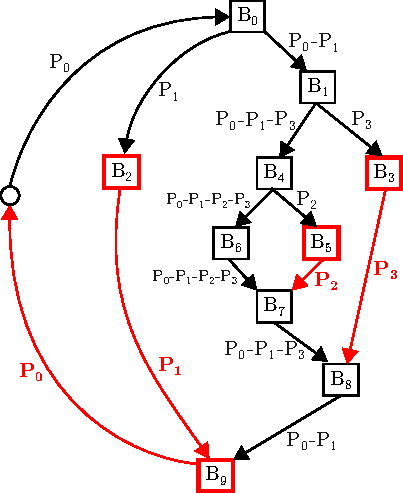
\includegraphics[scale=0.75]{figs/cfg-example.pdf}\\\vspace{1ex}
  \resizebox{0.45\textwidth}{!}{
  %\scalebox{0.8}{
     \begin{minipage}{0.5\textwidth}
     Instrumented value for each probe $P_i$:
     \begin{align*}
     \omega(P_0) &= w(B_0) + w(B_1) + w(B_4) + w(B_6) + w(B_7) + w(B_8) + w(B_9)\\
     \omega(P_1) &= w(B_2) - w(B_1) - w(B_4) - w(B_6) - w(B_7) - w(B_8)\\
     \omega(P_2) &= w(B_5) - w(B_6)\\
     \omega(P_3) &= w(B_3) - w(B_4) - w(B_6) - w(B_7)
     \end{align*}
     \end{minipage}
  }
}
  \caption{Example of a CFG with its maximum spanning tree in black. Basic blocks and edges highlighted in red are instrumented.
    Instrumenting them is enough for calculating the total work performed by the whole CFG.}
  \label{fig:cfg-example}
\end{figure}

In contrast to the naive instrumentation where each basic block records only its own amount of work, with the optimal profiling the work
counter increments needs to take other basic blocks into account. Figure~\ref{fig:cfg-example} shows an example CFG, where the instrumented
blocks are marked with red. In this example, executing block $B_3$ implies also executing $B_1$ and not executing $B_4$. We compute the
aggregated value of work for each probe in two steps: \textit{(i.)} we propagate information about the probes through the edges of the CFG,
as symbolic expressions, and then \textit{(ii.)} we use these edge flows to compose the aggregated value of the probes.

The symbolic expressions in the edges can then be used to compose the aggregated
value of the probes.
These symbolic expressions describe the probes that are in the same path of the
edge (positive terms) and those that are in complementary paths (negative
terms).
Therefore, the positive terms in the summed symbolic expression of a
basic block indicate that the amount of work of this basic block will be
incremented in the probes represented by these positive terms.
Similarly, the negative terms indicate that the amount of work of this basic block
will be decremented in the probes represented by these negative terms.
For example, because the symbolic expression for the basic block $B_8$ is $P_0 - P_1$,
the amount of work of $B_8$, denoted by $w(B_8)$, is incremented in probe $P_0$
and decremented in $P_1$.

\paragraph{Populating the edge flows:}
Intuitively, if all the edge flows are known for the complement of a spanning tree
then at any leaf of the spanning tree there is only one unknown edge flow.
This unknown edge flow can be calculated by Kirchhoff's first law.
This process repeats as a bottom-up propagation until all the unknown edge flows
have been calculated.
This algorithm can be formally defined as a post-order traversal on the spanning
tree.
Let $G$ be the CFG.
This algorithm first initializes the edge flows $D_{(u,v)}$, for each edge
$(u,v)$ in the CFG, as follows:
\[
D_{(u,v)} \gets
\begin{cases}
    P_{(u,v)} & \quad \text{if edge $(u,v)$ has a probe $P_{(u,v)}$}\\
    0       & \quad \text{otherwise}
\end{cases}
\]
Afterwards, for each vertex $u\in G$, in a post-order traversal of the spanning tree,
we can use the Kirchhoff's first law and apply the following operations
in a symbolic fashion:
\[
\Sigma^+_u = \sum_{v\in N^+(u)} D_{(u,v)}
\]
\[
\Sigma^-_u = \sum_{v\in N^-(u)} D_{(v,u)}
\]
\[
\forall v\in N^+(u):  D_{(u,v)} \gets
\begin{cases}
    D_{(u,v)} & \quad \text{if $D_{(u,v)}\neq 0$}\\
    \Sigma^-_u - \Sigma^+_u       & \quad \text{otherwise}
\end{cases}
\]
\[
\forall v\in N^-(u):  D_{(v,u)} \gets
\begin{cases}
    D_{(v,u)} & \quad \text{if $D_{(v,u)}\neq 0$}\\
    \Sigma^+_u - \Sigma^-_u       & \quad \text{otherwise}
\end{cases}
\]

\paragraph{Composing the aggregated value of the probes:}
If $x$ is a symbolic expression, then $\kappa_P(x)$ represents the coefficient
of the term $P$ in $x$.
In our case, $\kappa_P(x)$ will belong to the set $\{-1,0,1\}$.
Then, for all probes $P$:
\[
\omega(P) = \sum_{u\in G} \kappa_P(\Sigma^+_u)w(u)
\]

\subsection{Relaxed Instrumentation}

Although the optimal instrumentation significantly reduces the profiling
overhead when compared to the naive instrumentation, from an average overhead
of 79\% to 13\%, in some critical cases, even the optimal instrumentation can
result in overheads of up to 60\% (see benchmark \texttt{adpcm\_d} in Figure~\ref{fig:overhead-O3}).
In order to further reduce the overhead in these critical cases, we propose a
relaxation strategy that offers a trade-off between accuracy and overhead.
While the optimal instrumentation places probes in edges that are
less likely to be executed, the relaxation removes probes that are
more likely to be executed but add little to the final work metric.

% \begin{figure}[h]
%   \centering
%   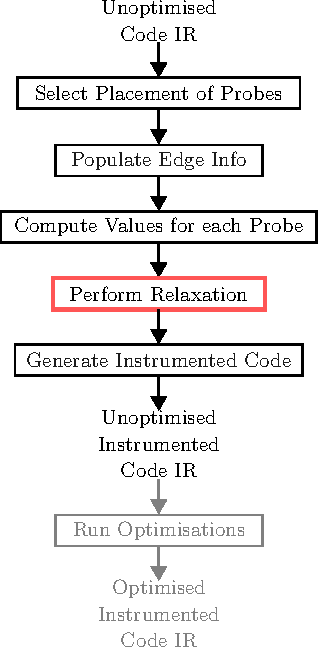
\includegraphics[scale=0.85]{figs/relax-instr-diagram.pdf}
%   \caption{Overview of the work instrumentation algorithm, including the relaxation technique.}
%   \label{fig:relax-instr-diagram}
% \end{figure}

%Figure~\ref{fig:relax-instr-diagram} shows an overview of the relaxed instrumentation algorithm.
%The highlighted step is introduced by the relaxed instrumentation on top of the previously defined optimal profiling.
The relaxation strategy performs a post processing on the resulting instrumentation of the optimal algorithm.
This post processing identifies probes that add little to the work metric, and removes their instrumentation.
In order to guarantee an upper bound for the dynamic error in the profiling measurement,
the relaxation algorithm applies a constrained post-processing on a per DAG (directed acyclic graph) basis.
By constraining the relaxation within each DAG by a maximum allowed static error,
it guarantees that the overall relaxation will also be constrained by the same bound.

The relaxation starts by extracting DAGs from the CFG.
First, the algorithm extracts all the subgraphs that represent a loop or the outer most region of the function.
Afterwards, these subgraphs are transformed into DAGs by ignoring the backedge
and also by considering that any loop within the subgraph is never executed,
i.e., only the headers of the inner loops are actually included into the DAG.
Figure~\ref{fig:cfg-relax-example} shows a CFG partitioned into two DAGs (consider
only basic blocks and edges completely inside the yellow and green boundaries).

\begin{figure}[t]
  \centering
  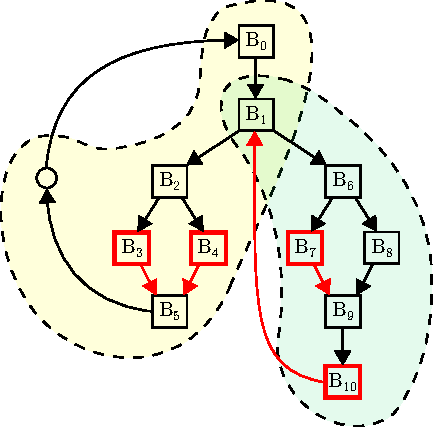
\includegraphics[scale=0.75]{figs/cfg-relax-example.pdf}
  \caption{Example of a CFG containing a loop and its decomposition into DAGs.
           The DAGs are the subgraphs within the dashed boundaries.}
  \label{fig:cfg-relax-example}
\end{figure}

%\begin{lstlisting}[caption={Optimal placement of probes for block frequency.}, label={lst:instrumentCFG}]
%// Input: CFG
%relaxInstrumentation(G) {
%  for loop in G:
%     DAG = colapseInnerLoops(loop)
%     relaxInstrumentedDAG(DAG)
%  DAG = colapseInnerLoops(G)
%  relaxInstrumentedDAG(DAG)
%}
%\end{lstlisting}

For every DAG with a set of probes $\{P_0, P_1, \ldots, P_k\}$,
we select a subset of the probes to be removed, subject to
the maximum allowed percentage error, $M$.
This strategy can be modeled as a 0-1 Knapsack problem:
\begin{gather*}
\textrm{max.}\quad\sum_{i=0}^{k} f(P_i)x_i,\quad
\textrm{s.t.}\quad\sum_{i=0}^{k} \varepsilon(P_i)x_i \leq M \\
x_i\in\{0,1\}, i\in\{0,\ldots,k\}
\end{gather*}
where $f(P_i)$ is the execution frequency of probe $P_i$, $x_i$ denotes the
probes selected for removal, and $\varepsilon(P_i)$ is the percentage error of
removing probe $P_i$ relative to the minimum work value possible to compute in
the DAG, i.e., if $m$ is the minimum amount of work possible to be computed when
executing the DAG, then $\varepsilon(P_i) = \frac{\omega(P_i)}{m}$.
Because the percentage error is computed based on the path with the minimum
amount of work, $\varepsilon(P_i)$ represents the maximum error possible that
would be incurred when removing probe $P_i$.
Furthermore, by constraining the percentage error of every DAG below a given
threshold, we guarantee that the final error of the relaxation will always be
bounded by the threshold.
% Furthermore, by constraining the percentage error of every DAG below a given threshold, we guarantee that the final error of the relaxation will always be bounded by the threshold, as demonstrated by Proposition~\ref{prop:relax-bound}.
%
% \begin{prop}\label{prop:relax-bound}
% Let $n_i$ be the number of times a given DAG $i$ is executed, $r_i$ be the total relaxation (amount of work removed) in DAG $i$, and $m_i$ be its minimum amount of work.
% If $\frac{r_i}{m_i} \leq M$ for every $i$,
% then the final error of the relaxation will always be bounded by the same threshold.
% \end{prop}
% \begin{proof}
% We can model the overall error of the relaxation as:
% \[
% 1 - \frac{n_1(m_1 - r_1) + n_2(m_2 - r_2) + \ldots + n_k(m_k - r_k) + c}{n_1m_1 + n_2m_2 + \ldots + n_km_k + c}
% \]
% That is,
% %\begin{equation*}
% \begin{gather*}
%  1 - \frac{n_1m_1 + n_2m_2 + \ldots + n_km_k + c}{n_1m_1 + n_2m_2 + \ldots + n_km_k + c} + \frac{n_1r_1 + n_2r_2 + \ldots + n_kr_k}{n_1m_1 + n_2m_2 + \ldots + n_km_k + c} = \\
%  \frac{n_1r_1 + n_2r_2 + \ldots + n_kr_k}{n_1m_1 + n_2m_2 + \ldots + n_km_k + c}
% \end{gather*}
% %\end{equation*}
% If $\frac{r_j}{m_j}$ is the maximum ratio $\frac{r_i}{m_i}$ for every $i$, then
% \begin{equation*}
% \begin{aligned}
%  \frac{n_1r_1 + n_2r_2 + \ldots + n_kr_k}{n_1m_1 + n_2m_2 + \ldots + n_km_k + c} &\leq\\
%  \frac{n_1r_j + n_2r_j + \ldots + n_kr_j}{n_1m_j + n_2m_j + \ldots + n_km_j + c} &\leq\\
%  \frac{n_1r_j + n_2r_j + \ldots + n_kr_j}{n_1m_j + n_2m_j + \ldots + n_km_j} &
% \end{aligned}
% \end{equation*}
% If $N = max\{n_i$ for every $i\}$, then
% \begin{equation*}
% \begin{aligned}
%  \frac{n_1r_j + n_2r_j + \ldots + n_kr_j}{n_1m_j + n_2m_j + \ldots + n_km_j} &\leq\\
%  \frac{Nr_j + Nr_j + \ldots + Nr_j}{Nm_j + Nm_j + \ldots + Nm_j} &=\\
%  \frac{Nkr_j}{Nkm_j} = \frac{r_j}{m_j} &\leq M
% \end{aligned}
% \end{equation*}
% \end{proof}


%\begin{lstlisting}[caption={Optimal placement of probes for block frequency.}, label={lst:instrumentCFG}]
%// Input: CFG
%relaxInstrumentedDAG(DAG){
%   P = ProbesIn(DAG)
%   m = minWork(DAG,P)
%   K = createKnapsackModel(P,m)
%   Bag = solveKnapsack(K)
%   for B in (P-Bag):
%     removeProbe(B)
%}
%\end{lstlisting}

%The necessary block-frequency information for optimising both the placement of
%probes can be acquired from profiles of previous executions of the program or by
%a static heuristic of the CFG during compilation.

For our experiments, we implemented two solvers for the 0-1 Knapsack problem:
the optimal brute-force solver and
the greedy heuristic based on sorting the items~\citep{dantzig57}.
We use the brute-force solver for DAGs with a small number of probes and the
greedy heuristic when the number of probes is greater than a threshold.
Some of the benchmarks have DAGs with several hundreds of probes, which could
result in a long compilation time.

\subsection{Whole Program Relaxation}

In this section we go one step even further.
In some cases, even the proposed relaxation strategy can still be conservative.
This conservatism can be overly restrictive in some cases, resulting in a
negligible overhead reduction but also causing just a negligible dynamic error
to the work profiling.
For these cases, we propose an adapted version of the relaxation algorithm that
operates on the whole program.
Traditionally, compiler optimizations are performed on the function-level, or at
best on a per module basis.
Whole program optimization (WPO) means that the compiler considers all
compilation units of the program and optimizes them using the combined knowledge
of how they are used together.

The \textit{whole program relaxation} works by using block-frequency profiling
from previous executions.
By having this profiling information, the whole program relaxation is able to
compute the error of removing a given probe in terms of the whole program's execution,
and then select a subset of all the probes to be removed.

For a program with a set of probes $\{P_0, P_1, \ldots, P_k\}$, we model the
whole program relaxation as the following 0-1 Knapsack problem:
\begin{gather*}
\textrm{max.}\quad\sum_{i=0}^{k} f(P_i)x_i,\quad
\textrm{s.t.}\quad\sum_{i=0}^{k} \varepsilon(P_i)x_i \leq M \\
x_i\in\{0,1\}, i\in\{0,\ldots,k\}
\end{gather*}
where $f(P_i)$ is the execution frequency of the instrumented basic block $P_i$,
$x_i$ denotes the probes selected for removal, $M$ is the error threshold, and
$\varepsilon(P_i)$ is the percentage error of removing probe $P_i$ relative to
the profiled global work, i.e.,
if $\Delta W$ is the work value for the whole program's execution, computed from
the basic block frequencies profiled from previous executions, the error for a
given probe $P_i$ is
\[
\varepsilon(P_i) = \frac{\omega(P_i)f(P_i)}{\Delta W}.
\]

Contrary to the per DAG relaxation, the whole program relaxation is not
guaranteed to be bounded by the error threshold $M$,
as it depends on the representativity % representativeness
of the profiling information provided to the whole program relaxation.

\section{Experimental Setup}\label{sec:setup}

\paragraph{Compiler and Hardware} We implemented our approach in LLVM 4.0.
We have made it available for download\footnote{Download URL hide for anonymous review.}.
Our evaluation platform has a quad-core 3.4 GHz Intel Core i7 CPU with 16 GB of RAM.
The operating system is openSUSE 42.2 with Linux kernel 4.4.27.

%The target platform is a Linux-4.4.27 system with an Intel Core i7-4770 3.40GHz Skylake~CPU with 16~GiB RAM.

\paragraph{Benchmarks}
We use a subset of the \textit{KDataSets} benchmark suite~\cite{chen10,chen12a},
shown in Table~\ref{tab:kdatasets}.
This suite provides 1,000 different inputs per benchmark.
The inputs have different sizes and often lead to different program execution paths.
%A summary of the benchmarks and their datasets is given in Table~\ref{tab:kdatasets}.
This benchmark suite allows us to evaluate our approach on a large number of inputs provided by independent
developers.


\begin{table}[t]
\centering
%\begin{subtable}{0.5\textwidth}
\scalebox{.8}{
\begin{tabular}{l|r|c|l}
\hline
\textbf{Program} & \textbf{LOC}    & \textbf{Input file size}            & \textbf{Input description}              \\ \hline % Domain
\rowcolor{gray!20}
bitcount      & 460    &  -                         & Numbers: random                \\ \hline
bzip2d        & 5125   & 0.2K-25M                   & Compressed files               \\ \hline
\rowcolor{gray!20}
bzip2e        & 5125   & 0.7K-57M                   & Files of any format            \\ \hline
crc32         & 130    & 0.6K-35M                   & Files of any format            \\ \hline
\rowcolor{gray!20}
dijkstra      & 163    & 0.06K-4.3M                 & Adjacency matrices             \\ \hline
ghostscript   & 99869  & 11K-43M                    & Postscript files               \\ \hline
\rowcolor{gray!20}
lame          & 14491  & 167K-36M                   & WAVE audios                    \\ \hline
mad           & 2358   & 28K-27M                    & MP3 audios                     \\ \hline
\rowcolor{gray!20}
patricia      & 290    & 0.6K-1.9M                  & IP and mask pairs              \\ \hline
stringsearch  & 338    &  0.1K-42M                 &  Text files                     \\ \hline
\end{tabular}
}
%\end{subtable}
\caption{Benchmarks used for calibrating the work model. Each program has a dataset of 1,000 inputs.}
\label{tab:kdatasets:training}

%\begin{subtable}{0.5\textwidth}
\scalebox{.8}{
\begin{tabular}{l|r|c|l}
\hline
\textbf{Program} & \textbf{LOC}    & \textbf{Input file size}            & \textbf{Input description}              \\ \hline % Domain
\rowcolor{gray!20}
adpcm\_c      & 210    & 167K-36M                   & WAVE audios                    \\ \hline
adpcm\_d      & 211    & 21K-8.8M                   & ADPCM audios                   \\ \hline
\rowcolor{gray!20}
jpeg\_c       & 14014  & 16K-137M                   & PPM images                     \\ \hline
jpeg\_d       & 13501  & 3.6K-1.5M                  & JPEG images                    \\ \hline
\rowcolor{gray!20}
qsort         & 154    & 32K-1.8M                   & 3D coordinates                 \\ \hline
rsynth        & 4111   & 0.1K-42M                   &  Text files                    \\ \hline
\rowcolor{gray!20}
sha           & 197    & 0.6K-35M                   & Files of any format            \\ \hline
susan\_c      & 1376   & 12K-46M                    & PGM images                     \\ \hline
\rowcolor{gray!20}
susan\_e      & 1376   & 12K-46M                    & PGM images                     \\ \hline
susan\_s      & 1376   & 12K-46M                    & PGM images                     \\ \hline
\rowcolor{gray!20}
tiff2bw       & 15477  & 9K-137M                    & TIFF images                    \\ \hline
tiffdither    & 15399  & 9K-137M                    & TIFF images                    \\ \hline
\rowcolor{gray!20}
tiffmedian    & 15870  & 9K-137M                    & TIFF images                    \\ \hline
tiff2rgba     & 15424  & 9K-137M                    & TIFF images                    \\ \hline
\end{tabular}
}
%\end{subtable}
\caption{Benchmarks used throughout our experimental evaluation.
         Each program has a dataset of 1,000 inputs.}
\label{tab:kdatasets}
\vspace{-1ex}
\end{table}



%Table~\ref{tab:kdatasets} gives the benchmarks used to train the cost model that is used for computing the instruction weights for
%the work metric. These were also used for collecting a fixed set of optimizations for the {\itercomp}. Table~~\ref{tab:kdatasets:test}
%lists the testing benchmarks used to evaluate our approach.


\paragraph{Performance Report}
We execute each benchmark with an input a number of times until the gap of the upper and lower confidence bounds is smaller than 5\% under
a 95\% confidence interval setting. We report the geometric mean performance across runs and inputs per benchmark, and provide a min-max
bar to show the variance across inputs.


\paragraph{The Set of Optimization Sequences}
For the purpose of evaluating the use of the work efficiency metric for guiding
online {\itercomp}, we collected in advance a fixed set of optimization sequences.
The reason for using this fixed set is to allow a direct comparison among the configurations.
We assume that a good generator of optimization sequences will be used in a real online scenario.
Having a better generator would only improve the whole process of the online {\itercomp}.
This set contains 500 optimization sequences collected in a random search using the training benchmarks.
These optimization sequences contain an average of 40 individual optimization passes,
including repetitions, with a maximum of 119 optimization passes, but it also contains
optimization sequences which consist of a single flag, such as the default optimizations
\texttt{-O1}, \texttt{-O2}, \texttt{-O3}, \texttt{-Os}, and \texttt{-Oz}.

All optimization sequences in the set of optimizations were generated completely
at random, without using any knowledge of individual transformations.
Each optimization sequence was generated in two steps: \textit{(1)} randomly
selects the number of flags; \textit{(2)} randomly selects the flags, allowing repetitions.
Afterwards, this randomly generated optimization sequence would be included in
the set of optimization sequences only if it was able to improve the performance
of a training benchmark, also selected at random, in respect of the \texttt{-O3}
default optimization.
This process was repeated until we obtained all the 500 distinct optimization sequences.

  % \begin{minipage}{0.9\textwidth}
  %    \vspace{1em}
  %    \noindent\textbf{Example of a short optimization sequence:}\vspace{-1ex}
  %    \justify{\flagstype -mem2reg -simplifycfg -constprop -dce}
  % \end{minipage}
  %
  % \begin{minipage}{0.9\textwidth}
  %    \vspace{1em}
  %    \noindent\textbf{Example of a long optimization sequence:}\vspace{-1ex}
  %    \justify{\flagstype -globalopt -reassociate -instcombine -loop-rotate -block-freq -deadargelim -early-cse -sroa -argpromotion -sccp -tbaa -barrier -constmerge \mbox{-loop-vectorize} -domtree -basicaa -memdep -basiccg -memcpyopt \mbox{-constprop} -adce -globaldce -mem2reg -constmerge \mbox{-globaldce} -constprop -instsimplify -dse -dce -simplifycfg -loop-unroll -reassociate -constprop \mbox{-globaldce} -instsimplify -adce -constmerge -bb-vectorize -dce -mergefunc -simplifycfg -dse -loop-unroll -globaldce}
  % \end{minipage}
  %
  % \begin{minipage}{0.9\textwidth}
  %    \vspace{1em}
  %    \noindent\textbf{Example of an optimization sequence which includes {-O3}:}\vspace{-1ex}
  %    \justify{\flagstype -O3 -adce -globaldce -simplifycfg -memcpyopt -reassociate -mergefunc \mbox{-dce} -dse}
  %    \vspace{2em}
  % \end{minipage}

%Repeating the same optimization pass can be beneficial and usually expected by other passes.
%For example, the {\flagstype -loop-simplify} pass is used for transforming loops into a canonical form by inserting pre-header and exit basic blocks.
%Although this pass inserts jumps due to redundant basic blocks, this canonical form can be favourable to other loop optimizations.
%Because of the redundant basic blocks, this optimization pass expects that the {\flagstype -simplifycfg} will eventually be executor later on the optimization pipeline.
%Another example of such inter-relation between transformations concerns the {\flagstype -licm} and {\flagstype -mem2reg} passes.
%The {\flagstype -licm} pass is responsible for moving invariant code out from the loop body.
%It usually creates new local variables, using memory access operations, for assisting with the code manipulation, which means that the executing the {\flagstype -mem2reg} pass afterwards would be useful as a cleanup pass for removing the extra memory accesses generated.
%However, many of the analysis required for identifying loop invariant also benefit from the transformations performed by the {\flagstype -mem2reg} pass.
%These examples illustrate the importance of repeating optimization passes.
%Moreover, they illustrate the intricate relation amongst several transformations.

\section{Experimental Results}\label{sec:results}

In this section we discuss our experimental evaluation of the work profiling strategies and
the effectiveness of the work efficiency metric on guiding true online {\itercomp}.
We use the following naming convention for the profiling strategies considered
throughout this section:
\begin{itemize}[leftmargin=3mm]
\item \textbf{\OracleRM} measures the actual speedup over the unoptimized version of the program for any given input. In our experiments,
    this oracle is allowed to execute each input \emph{at least twice} so the speedup can be computed.
\item \textbf{\OraclePP} measures the work efficiency metric with a \textit{magically perfect} non-intrusive profiling.
  Because this version simulates a \textit{perfect} profiling, with zero overhead,
  it allows us to isolate and evaluate the actual effectiveness of the work efficiency metric.
\item \textbf{\OptProf} corresponds to the work profiling using the optimal placement of the probes. This profiling strategy requires
    \emph{a single execution} of the program for any given input.
\item \textbf{\WCRelax-\textit{N}\%} measures the work efficiency metric using the work profiling with a \textit{N}\% threshold for
the \WCRelaxLower relaxation.
  Similar to the \OptProf, this profiling strategy also requires a single execution of the program for any given input.
\item \textbf{\WPRelax-\textit{N}\%} is similar to the \WCRelax, but it applies the \WPRelaxLower relaxation instead.
\end{itemize}

\begin{figure*}[t!]
    \centering
    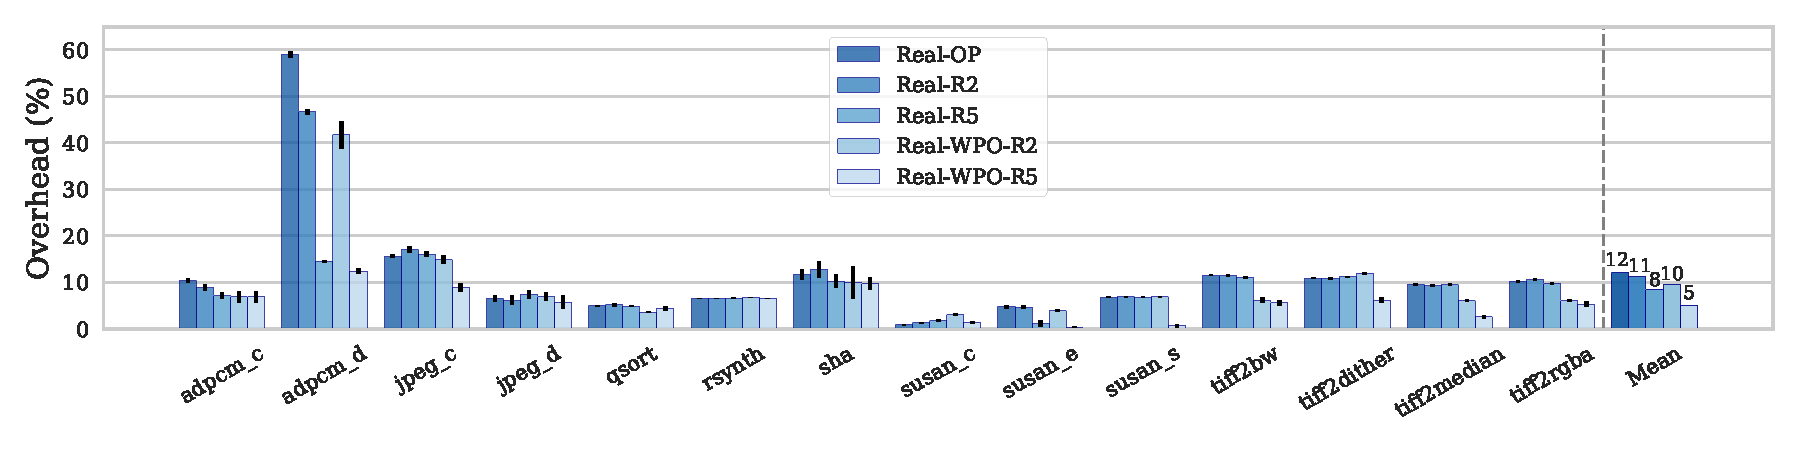
\includegraphics[width=\textwidth]{figs/overhead-O3.pdf}
    \caption{Instrumentation overhead for each benchmark averaged over all inputs, when compiled with {\flagstype -O3}.}
    \vspace{-3mm}
    \label{fig:overhead-O3}
\end{figure*}

\begin{figure*}[t!]
    \centering
    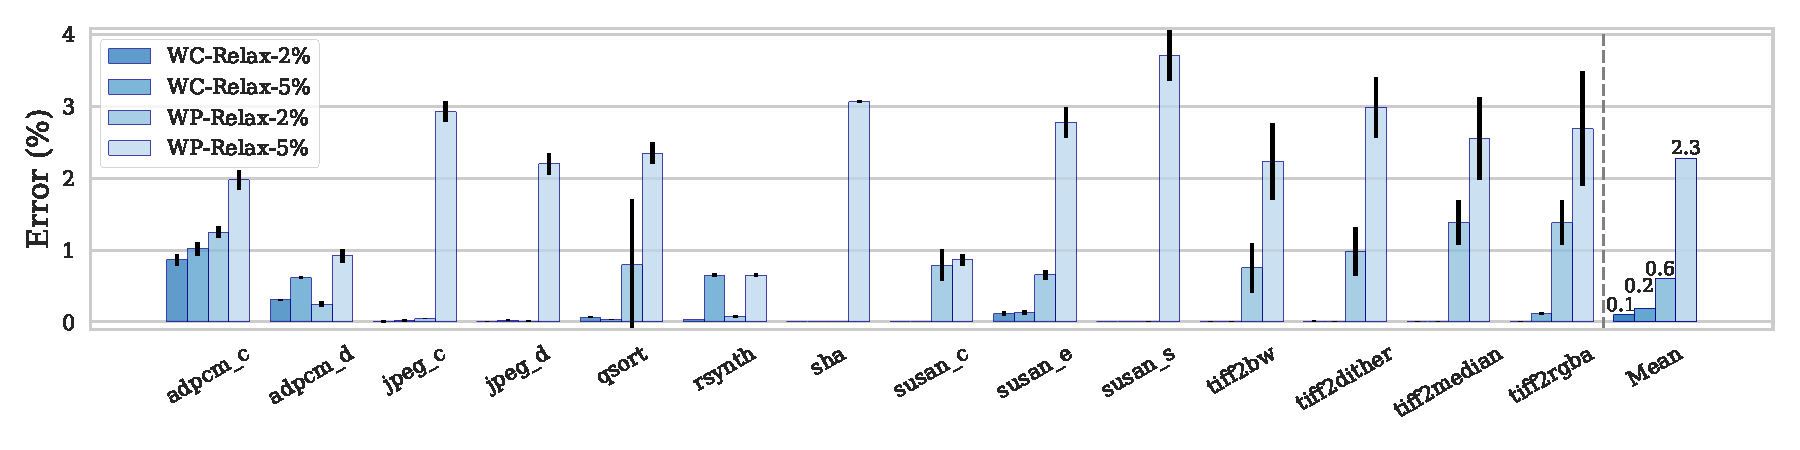
\includegraphics[width=\textwidth]{figs/error-O3.pdf}
    \caption{Dynamic error of the work profiling averaged over the 1000 inputs, after relaxing the number of probes.}
    \vspace{-3mm}
    \label{fig:error-O3}
\end{figure*}

\subsection{Evaluation of the Instrumentation}

First, we evaluate the runtime overhead introduced by the work efficiency profiling. A high overhead would impact the user's experience
and would make our approach impractical. We take the original and instrumented versions of each benchmark, we compile them using the
baseline \texttt{-O3} setting, and execute them with all 1,000 inputs. The difference in their runtimes, for the same input, is the
instrumentation overhead. Figure~\ref{fig:overhead-O3} shows the average overhead for each benchmark and work profiling strategy.

\OptProf typically slows the application down by 10\%, noticeably affecting the user experience, while in the worst case its overhead
reaches 59\%. It is clearly unsuitable for online work profiling. \WCRelax and \WPRelax fare better, especially when used with a higher
5\% threshold. \WPRelax-\textit{5}\%, in particular, has an average overhead of only 5\%, 13\% in its worst case.

For almost all the profiling strategies, their worst case is \texttt{adpcm\_d}. Still, compared to the 59\% overhead of the \OptProf,
\WCRelax-\textit{5}\% and \WPRelax-\textit{5}\% incur only about a quarter of that overhead. This benchmark has a single hot function
consisting mainly of a single hot loop with several branches inside it. Most of the overhead comes from two probes which are placed in
very frequently executed blocks but contribute little to the total work of the loop. The maximum possible error caused by removing either
of the probes, based on the analysis of the DAG, is about 1.3\%. Both relaxation strategies identify this opportunity and remove the probes.

Some benchmarks display unexpectedly higher overheads under the relaxation strategies. This is counter-intuitive because relaxation only
reduces the number of instrumented probes without changing their placement. By analyzing these cases, we noticed that we could not remove
the most frequently executed probes, so relaxation had little positive impact. At the same time, we removed some probes which were
infrequently executed but were taken into consideration by the LLVM optimization heuristics. In some cases, removed probes caused different
and suboptimal decisions to be made, very slightly increasing the runtime.

Figure~\ref{fig:error-O3} shows that profiling with relaxation incurs very little dynamic error. It also confirms that the \WCRelaxLower
relaxation is overly conservative, while the \WPRelaxLower relaxation achieves a better trade-off. Although the error bound is not
guaranteed by the \WPRelaxLower relaxation, its dynamic error is always below 5\%. For both relaxation strategies the 2\% threshold is too
conservative to be useful. The rest of the paper only evaluates the 5\% threshold.

\subsection{Evaluation of Online {\IterComp}}

\begin{figure*}[t]
    \centering
    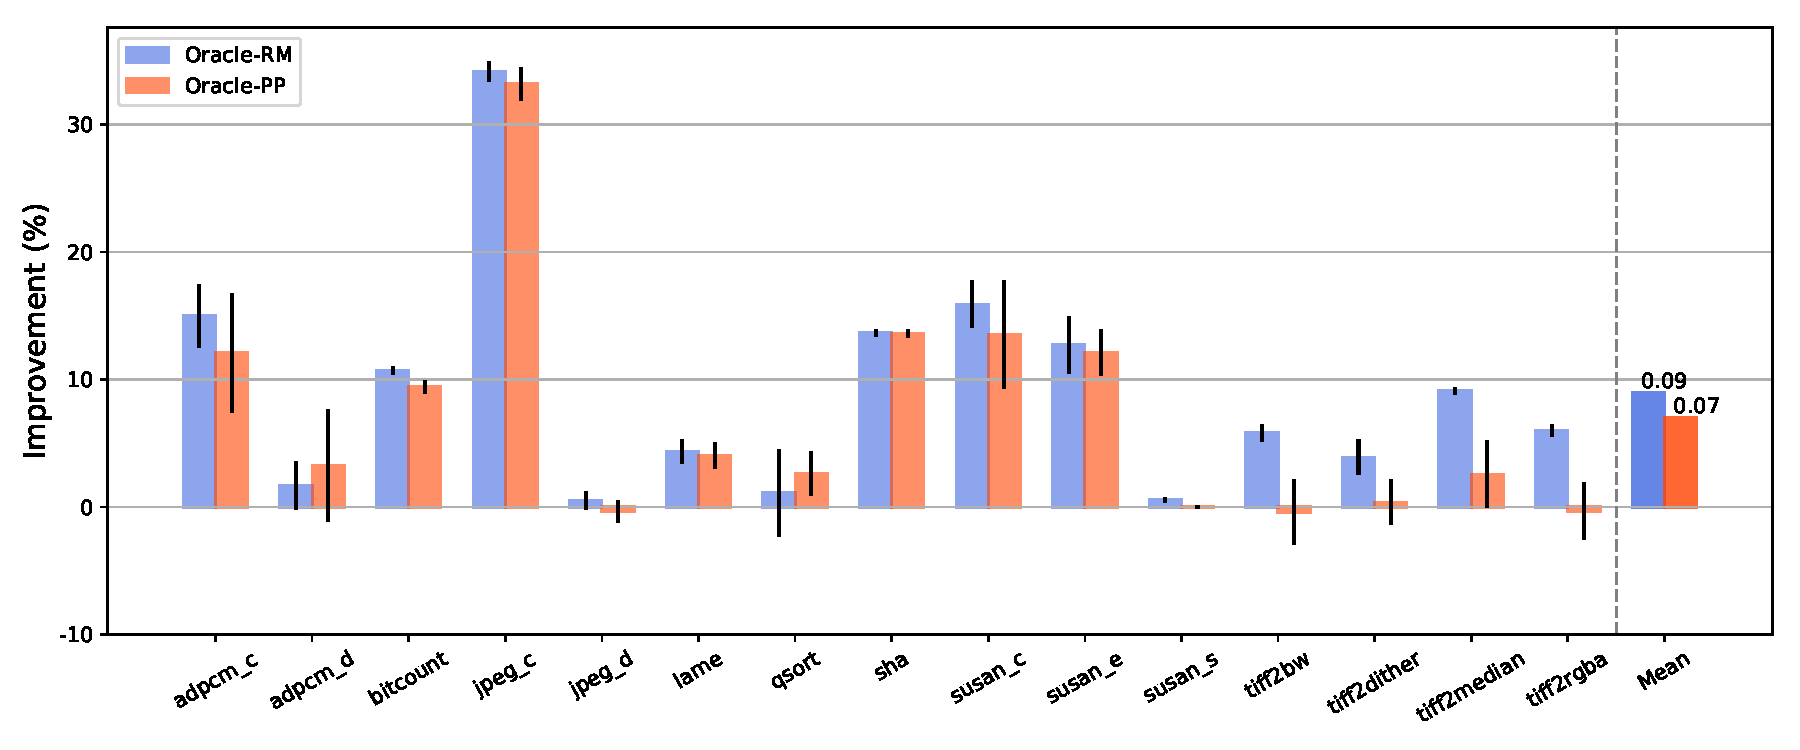
\includegraphics[width=\textwidth]{figs/speedups.pdf}
    \caption{Speedups obtained from the final optimization sequence selected by the online {\itercomp}.
             The speedups reported for each benchmark represents the average speedup across their complete 1000 input datasets.}
    \label{fig:speedups}
\end{figure*}

In this section we evaluate the effectiveness of our work efficiency metric. We perform online {\itercomp} using all five profiling
strategies, namely \OracleRM, \OraclePP, \OptProf, \WCRelax-5\%, and \WPRelax-5\%. We evaluate every optimization sequence on multiple
inputs. We use work efficiency to rank different optimization sequences and we select the one with the highest work efficiency.

\OracleRM makes iterative compilation decisions based on the actual speedup over the unoptimized version. It does not depend on any kind of
instrumentation or work estimation, so it acts as the baseline against which the rest of the profiling strategies are compared. \OraclePP
is also not affected by instrumentation but uses work efficiency instead of speedup. We use it to decide whether our work metric can be
used for iterative compilation on principle. The other configurations demonstrate the viability of applying online {\itercomp} in
real-world scenarios.

We evaluate the quality of the selected optimization sequences by comparing their average speedup over \texttt{-O3} across all 1,000 inputs
of each benchmark.
Figure~\ref{fig:speedups} shows these speedups for all test benchmarks. In most cases, \OraclePP is very close to \OracleRM, achieving on
average 80\% of its speedup. This demonstrates that it is a valid choice to drive iterative compilation decision using work efficiency. The
few cases where the two strategies produce noticeably different results are for the \texttt{tiff} benchmarks. The weaker correlation between
work and unoptimized runtime for these benchmarks is to blame for the lower speedups achieved by \OraclePP.

The \OptProf achieves 4\% improvement on average, which represents a little bit more that half of the speedup of \OraclePP. The culprit is
the one thing that is different between the two strategies, the profiling instrumentation. It affects the search in two key ways:
\textit{(i.)} the overhead incurred by profiling affects the execution time and, through it, the work efficiency metric,
\textit{(ii.)} the inserted instrumentation code occasionally changes how optimizations are applied, e.g., due to the use of a global
variable or in decisions taken based on a cost-model for the instructions. With the \OptProf configuration, instrumentation is very
intrusive and this translates into lower speedups or even slowdowns for five benchmarks. Just measuring work with traditional profiling
approaches is not enough for online iterative compilation.

This is where our two relaxation algorithms become particularly important. Beyond just reducing the user perceived overhead of iterative
compilation, they also improve the search itself by keeping the behavior of the instrumented binary as close as possible to that of the
uninstrumented one. Relaxation reduces the deleterious effects of instrumentation on both the runtime and how optimizations are applied.
As a result, \WCRelax-5\% and \WPRelax-5\% are very close to the behavior of \OraclePP and they achieve about 60\% of the performance
improvement obtained by \OracleRM.

\begin{figure*}[t]
  \centering
  \subfigure[\OptProf]{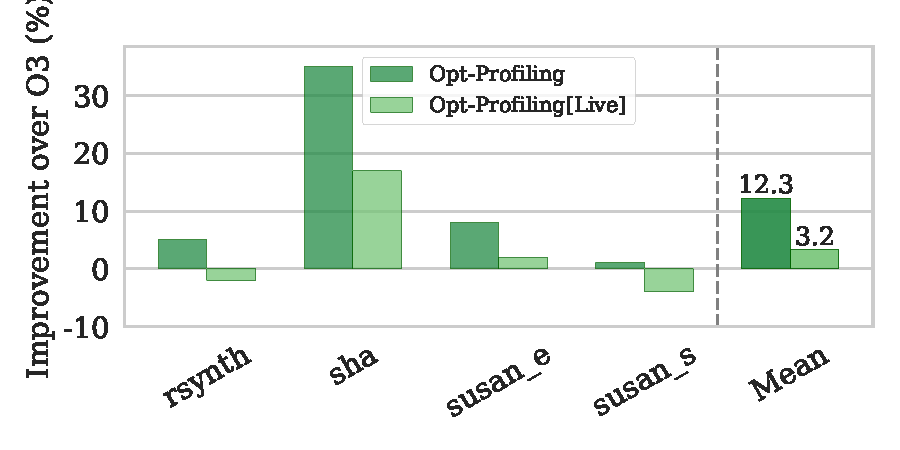
\includegraphics[width=0.3\textwidth]{figs/Opt-Profiling-deployment.pdf}}
  \hfill
  \subfigure[\WCRelax-5\%]{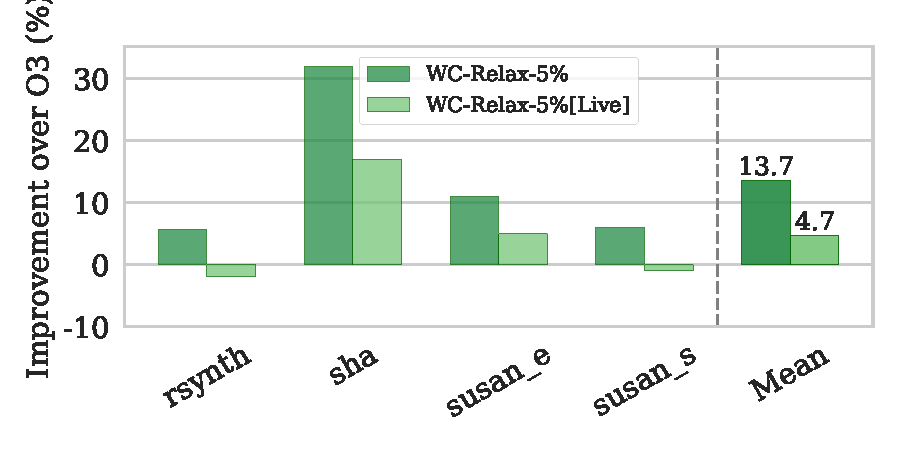
\includegraphics[width=0.3\textwidth]{figs/WC-Relax-5-deployment.pdf}}
  \hfill
  \subfigure[\WPRelax-5\%]{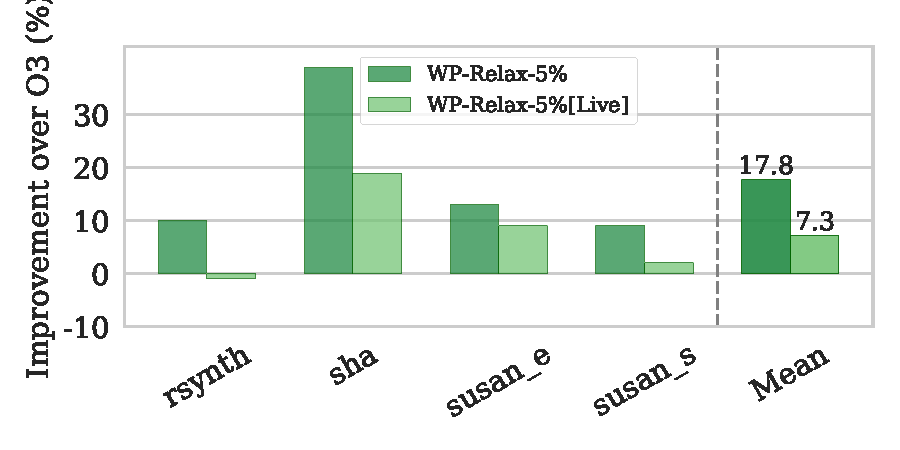
\includegraphics[width=0.3\textwidth]{figs/WP-Relax-5-deployment.pdf}}
  \caption{Speedup over \texttt{-O3} for the best optimization selected by the search, as well as the average speedup as experienced by the
    user throughout the search process ([Live]). The results show that the proposed approach is profitable in real-world online scenarios.}
  \label{fig:deployment_cost}
\end{figure*}

\subsection{Overall Benefit of Online Search}\label{subsec:search}

A typical argument against online adaptive techniques is that the overhead of management and the slowdown due to testing suboptimal
configuration might overshadow the benefits of the technique. In this subsection, we establish that online iterative compilation is
profitable even when factoring in the online costs. We modify the architecture described in Section~\ref{sec:oic-infra} to make it more
realistic by using genetic search~\cite{knijnenburg02,kulkarni04} over the whole space of possible optimizations. 

Figure~\ref{fig:deployment_cost} shows, for each benchmark and configuration, the speedup over \texttt{-O3} of the best optimization sequence
evaluated by the search but also the average profitability/cost experienced by the user throughout the search process (labeled as [Live]),
which takes into account the overhead of the work profiling. We evaluate three configurations that use work profiling, namely \OptProf,
\WCRelax-5\%, and \WPRelax-5\%. By widening the search space, we are able to improve performance significantly compared to the results in
Figure~\ref{fig:speedups}. In terms of the overall speedup throughout the search, all three configurations are profitable on average. 
Although there is a slight risk we select a suboptimal version and the user experiences slowdown, our genetic search focuses on promising
optimization sequences, reducing the risk of selecting a suboptimal version of the program as the genetic population evolves. For all three
configurations, after the first generation, the optimization sequences we evaluate tend to overcome this issue, with their benefits
surpassing the profiling overheads. This is particularly true for \WPRelax-5\%, where the small overhead combined with the large speedup
lead to a 7.3\% overall speedup.

\section{Related Work}\label{sec:relatedwork}

\subsection{{\IterComp}}
Multiple different adaptive compilation techniques have been proposed for finding a near optimal combination of optimization
settings~\cite{agakov06,hoste2008cole,kulkarni04,stephenson03} by probabilistically searching the space of possible combinations. But with
all of them there is uncertainty about whether the quality of their results depends on the data set used. Chen~\etal~\cite{chen10,chen12a}
examined this issue and showed that indeed the best optimization options differ across inputs. Still, in most cases it is possible to find
a combination of optimizations that produces good results across all inputs, by using a few tens of inputs to evaluate our optimizations
on. While a positive result, this is still impractical. Producing tens of realistic input sets might be difficult. Even if not, each
combination of optimization options has to be evaluated on every input set, increasing the time \itercomp takes by at least an order of
magnitude.

Recent research~\cite{chen12b,fang15} has used real data for performing online {\itercomp} on distributed data center applications. Each
worker receives a subset of the input dataset to evaluate a small set of optimization settings on. The best such setting from each round
is used for subsequent executions of the same code. By testing new settings and re-evaluating old ones on new datasets this approach makes
it more likely to select an optimization setting that works well across inputs. Like in~\cite{chen10} every setting is tested on the same
set of inputs, wasting time and energy. This approach only works well with MapReduce-like workloads, since it relies on the MapReduce
framework for repeating the same computation multiple times without side-effects or corrupting the input.

Fursin~\etal~\cite{fursin07} attempted to find a more general approach for online \itercomp. They proposed instructions per cycle (IPC) as
a metric for comparing runs of the same program with different optimization settings and different inputs: application binaries displaying
higher IPC are more efficient than lower IPC binaries. Their results show that IPC seems promising as a robust metric for {\itercomp}.
However, some optimization techniques affect IPC in the opposite way, making the program more efficient while lowering IPC. In the context
of multithreaded application, IPC cannot be used to estimate performance~\cite{alameldeen06,eyerman08}. Aalameldeen and
Wood~\cite{alameldeen06} suggest a work metric for quantifying efficiency, but choosing a unit of work is program specific and challenging.

%\subsection{Work and Input Size Metrics}

%Previous work have proposed profiling-based mechanism to estimate input sizes~\cite{zaparanuks12,coppa14}.
%Coppa~\etal~\cite{coppa14} in particular propose the concept of \textit{read memory size} for automatically estimating the size of the input passed to a routine, where \textit{read memory size} represents the number of distinct memory cells first accessed by a read operation.
%In other words, the \textit{read memory size} metric measures the size of the useful portion of the input's memory footprint.
%However, because we are interested in the amount of computational work performed in respect of a given input, the memory footprint of the input may not always have a direct correspondence to  the amount of computational work.

%Goldsmith~\etal~\cite{goldsmith07} use \textit{block frequency} as the measure for performance for empirically describing the asymptotic behavior of programs, which is known as empirical computational complexity.
%Block frequency is a relative metric that represents the number of times a basic block executes~\cite{ball94,ball96}.
%They argue in favor of block frequency due to its portability, repeatability and exactness, since it does not suffer from timer resolution problems or non-deterministic noises.
%Block frequency also has the advantage of being efficiently profiled by means of automatic code instrumentation~\cite{knuth73,ball94}.

%However, in the context of comparing different optimizations, although block frequency would be able to capture aspects of optimizations that simplify the control-flow graph (CFG), measuring work at the basic block resolution would not capture effects of optimizations at the instruction level.
%Because of that, we extend the idea of using basic block frequency to measure computational work by also considering the computational cost of each basic block.
%The computational cost of a basic block is given by weighing the instructions that it contains.

\subsection{Optimal Instrumentation}

Donald Knuth~\cite{knuth73} introduced an optimal algorithm for profiling block frequency, inserting much fewer probes than naive
instrumentation approaches that were used in practice~\cite{knuth71}. Forman~\cite{forman81} proposed further overhead reductions by
placing the probes in basic blocks that are less likely to be executed based on static heuristics. Ball and Larus~\cite{ball94} offered a
detailed discussion comparing two approaches for optimally profiling block frequency, namely, placing probes on the vertices or the edges
of the control-flow graph (CFG). They show that the edge-based approach produces optimal placement of probes. Theirs is the algorithm we
used for our initial selection of probes before relaxation.

\section{Conclusions}
This paper has introduced a novel efficiency metric which enables us to compare in terms of performance versions of an application compiled
in different ways even when they perform different amounts of work. Our approach automatically estimates the work done by each basic block
of the application and inserts instrumentation code to increment a global work counter every time a block is executed. We optimize the
placement of the instrumentation probes to reduce the runtime overhead. On top of it, we implement two strategies for removing probes from
the application to control the trade-off between runtime overhead and work estimation accuracy.

We use this efficiency metric to enable for the first time true online iterative compilation. Instead of comparing different optimizations
sequences offline by running the application repeatedly with different optimizations applied but the same input, we can now compare runs
using different inputs as they are provided by the user. We evaluated our online iterative compilation methodology using the KDataSets
benchmark suite. Experimental results show that we deliver \red{80\%} of the speedup achieved by an offline oracle while not having to
execute any input more than once. Our probe optimization and removal strategies bring the instrumentation overhead down to only \red{4\%}
on average, making our approach suitable for integration into software products.


%This paper has presented a novel work efficiency metric to enable one to compare the performance of any two different compiled versions of
%a program without executing a given input more than once. This ability allows us to implement, for the first time, a true online iterative
%compilation  to search for the best compilation options  based on actual user inputs seen in the deployment environment.

%We develop a compiler-based, low-overhead instrumentation mechanism to gather the require data to evaluate the work metric. Our mechanism
%does this without any human involvement. We show that by carefully selecting where to place the probes in the source code, the
%instrumentation overhead can be negligible. We give two probe optimization strategies, allowing developers to balance the instrumentation
%overhead and the performance error.


%We  evaluate our approach using the KDataSets benchmark suit. Experimental results show that our approach delivers \red{80\%} of the
%speedup achieved by an offline  oracle, but without executing any input more than once. We show that our probe optimization strategy is
%highly effective, which brings the instrumentation overhead down to only \red{4\%} on average, making our approach practical for regular
%use.

%Our proposed technique for relaxed instrumentation can also be applied for similar profiling scenarios, such as profiling empirical
%computational complexity~\cite{goldsmith07,zaparanuks12,coppa14}.


%
%\section*{Acknowledgments}
%
%This work was supported by the UK Engineering
%and Physical Sciences Research Council (EPSRC) under grants
%EP/L01503X/1 for the University of Edinburgh, School
%of Informatics, Centre for Doctoral Training in Pervasive
%Parallelism, % (\url{http://pervasiveparallelism.inf.ed.ac.uk/}),
%and also by the Institute for Computing Systems Architecture (ICSA)
%in the School of Informatics at the University of Edinburgh.

\bibliographystyle{ACM-Reference-Format}
\bibliography{bibliography}

\end{document}
